\begin{filecontents*}{\jobname.bib}
% =========================================================================
% Agentic Mesh — IEEE-Ordered Bibliography (1..26 by First Appearance)
% =========================================================================

% [1]
@article{satyanarayanan2017emergence,
  author={Satyanarayanan, Mahadev},
  title={The Emergence of Edge Computing},
  journal={Computer},
  volume={50},
  number={1},
  pages={30--39},
  year={2017},
  publisher={IEEE}
}

% [2]
@article{brewer2012cap,
  author={Brewer, Eric},
  title={{CAP} Twelve Years Later: How the ``Rules'' Have Changed},
  journal={Computer},
  volume={45},
  number={2},
  pages={23--29},
  year={2012},
  publisher={IEEE}
}

% [3]
@article{corbett2013spanner,
  author={Corbett, James C. and Dean, Jeffrey and Epstein, Michael and Fikes, Andrew and Frost, Christopher and Furman, J. J. and Ghemawat, Sanjay and Gubarev, Andrey and Heiser, Christopher and Hochschild, Peter and others},
  title={Spanner: {Google}'s Globally Distributed Database},
  journal={ACM Transactions on Computer Systems},
  volume={31},
  number={3},
  pages={1--22},
  year={2013},
  publisher={ACM}
}

% [4]
@inproceedings{ongaro2014raft,
  author={Ongaro, Diego and Ousterhout, John},
  title={In Search of an Understandable Consensus Algorithm},
  booktitle={Proc. 2014 USENIX Annual Technical Conference (ATC)},
  pages={305--319},
  year={2014}
}

% [5]
@article{gilbert2002brewer,
  author={Gilbert, Seth and Lynch, Nancy},
  title={Brewer's Conjecture and the Feasibility of Consistent, Available, Partition-Tolerant Web Services},
  journal={ACM SIGACT News},
  volume={33},
  number={2},
  pages={51--59},
  year={2002},
  publisher={ACM}
}

% [6]
@inproceedings{decandia2007dynamo,
  author={DeCandia, Giuseppe and Hastorun, Deniz and Jampani, Madan and Kakulapati, Gunavardhan and Lakshman, Avinash and Pilchin, Alex and Sivasubramanian, Swaminathan and Vosshall, Peter and Vogels, Werner},
  title={Dynamo: {Amazon}'s Highly Available Key-Value Store},
  booktitle={Proc. 21st ACM Symposium on Operating Systems Principles (SOSP)},
  pages={205--220},
  year={2007},
  publisher={ACM}
}

% [7]
@article{codd1970relational,
  author={Codd, Edgar F.},
  title={A Relational Model of Data for Large Shared Data Banks},
  journal={Communications of the ACM},
  volume={13},
  number={6},
  pages={377--387},
  year={1970},
  publisher={ACM}
}

% [8]
@article{bailis2014coordination,
  author={Bailis, Peter and Fekete, Alan and Franklin, Michael J. and Ghodsi, Ali and Hellerstein, Joseph M. and Stoica, Ion},
  title={Coordination Avoidance in Database Systems},
  journal={Proc. of the VLDB Endowment},
  volume={8},
  number={3},
  pages={185--196},
  year={2014}
}

% [9]
@inproceedings{yao2023react,
  author={Yao, Shunyu and Zhao, Jeffrey and Yu, Dian and Du, Nan and Shafran, Izhak and Narasimhan, Karthik and Cao, Yuan},
  title={{ReAct}: Synergizing Reasoning and Acting in Language Models},
  booktitle={Proc. International Conference on Learning Representations (ICLR)},
  year={2023}
}

% [10]
@article{ji2023hallucination,
  author={Ji, Ziwei and Lee, Nayeon and Frieske, Rita and Yu, Tiezheng and Su, Dan and Xu, Yan and Ishii, Etsuko and Bang, Ye Jin and Madotto, Andrea and Fung, Pascale},
  title={Survey of Hallucination in Natural Language Generation},
  journal={ACM Computing Surveys},
  volume={55},
  number={12},
  pages={1--38},
  year={2023},
  publisher={ACM}
}

% [11]
@inproceedings{singh2025llmtexttosql,
  author={Singh, Aditi and Shetty, Akash and Ehtesham, Abul and Kumar, Saket and Khoei, Tala Talaei},
  title={A Survey of Large Language Model-Based Generative {AI} for Text-to-{SQL}: Benchmarks, Applications, Use Cases, and Challenges},
  booktitle={Proc. 2025 IEEE 15th Annual Computing and Communication Workshop and Conference (CCWC)},
  pages={15--21},
  year={2025},
  doi={10.1109/CCWC62904.2025.10903689}
}

% [12]
@article{hipp2020sqlite,
  author={Hipp, D. Richard and Kennedy, Dan and Mistachkin, Joe},
  title={{SQLite}: An Embeddable, Zero-Configuration {SQL} Database Engine},
  journal={SQLite Development Team},
  year={2020}
}

% [13]
@article{trautwein2022libp2p,
  author={Trautwein, Dennis and Raman, Aravind and Tyson, Gareth and Castro, Ignacio and Sathiaseelan, Arjuna},
  title={Design and Evaluation of libp2p: A Modular Network Stack for Peer-to-Peer Applications},
  journal={IEEE/ACM Transactions on Networking},
  volume={31},
  number={4},
  pages={1550--1565},
  year={2022},
  publisher={IEEE}
}

% [14]
@inproceedings{vyzovitis2020gossipsub,
  author={Vyzovitis, Dimitris and Napier, Yiannis and McCormick, David and Jerger, Jeromy and Dias, David},
  title={{GossipSub}: An Extensible Baseline Pubsub Protocol for libp2p},
  booktitle={2020 IEEE International Conference on Blockchain and Cryptocurrency (ICBC)},
  pages={1--9},
  year={2020},
  organization={IEEE}
}

% [15]
@article{fidge1988timestamps,
  author={Fidge, Colin J.},
  title={Timestamps in Message-Passing Systems That Preserve the Partial Ordering},
  journal={Australian Computer Science Communications},
  volume={10},
  number={1},
  pages={56--66},
  year={1988}
}

% [16]
@article{lamport1978time,
  author={Lamport, Leslie},
  title={Time, Clocks, and the Ordering of Events in a Distributed System},
  journal={Communications of the ACM},
  volume={21},
  number={7},
  pages={558--565},
  year={1978},
  publisher={ACM}
}

% [17]
@article{lamport1998part,
  author={Lamport, Leslie},
  title={The Part-Time Parliament},
  journal={ACM Transactions on Computer Systems},
  volume={16},
  number={2},
  pages={133--169},
  year={1998},
  publisher={ACM}
}

% [18]
@inproceedings{terry1995managing,
  author={Terry, Douglas B. and Theimer, Marvin M. and Petersen, Karin and Demers, Alan J. and Spreitzer, Mike J. and Hauser, Carl H.},
  title={Managing Update Conflicts in {Bayou}, a Weakly Connected Replicated Storage System},
  booktitle={Proc. 15th ACM Symposium on Operating Systems Principles (SOSP)},
  pages={172--182},
  year={1995},
  publisher={ACM}
}

% [19]
@inproceedings{kleppmann2019local,
  author={Kleppmann, Martin and Wiggins, Adam and van Hardenberg, Peter and McGranaghan, Mark},
  title={Local-First Software: You Own Your Data, in Spite of the Cloud},
  booktitle={Proc. 2019 ACM SIGPLAN International Symposium on New Ideas, New Paradigms, and Reflections on Programming and Software (Onward!)},
  pages={154--178},
  year={2019},
  publisher={ACM}
}

% [20]
@inproceedings{shapiro2011conflict,
  author={Shapiro, Marc and Pregui{\c{c}}a, Nuno and Baquero, Carlos and Zawirski, Marek},
  title={Conflict-Free Replicated Data Types},
  booktitle={Proc. 13th International Symposium on Stabilization, Safety, and Security of Distributed Systems (SSS)},
  pages={386--400},
  year={2011},
  publisher={Springer}
}

% [21]
@misc{vanderheide2023crsqlite,
  author={van der Heide, Matt},
  title={{cr-sqlite}: Convergent, Replicated, Eventual-Consistent {SQLite}},
  year={2023},
  howpublished={\url{https://github.com/vlcn-io/cr-sqlite}}
}

% [22]
@misc{schoppmann2022rqlite,
  author={Schoppmann, Philip},
  title={{rqlite}: The Lightweight, Distributed Relational Database Built on {SQLite}},
  year={2022},
  howpublished={\url{https://github.com/rqlite/rqlite}}
}

% [23]
@misc{electricsql2023,
  author={{ElectricSQL Team}},
  title={{ElectricSQL}: Local-First Sync Layer for Modern Apps},
  year={2023},
  howpublished={\url{https://electric-sql.com}}
}

% [24]
@article{demers1987epidemic,
  author={Demers, Alan and Greene, Dan and Hauser, Carl and Irish, Wes and Larson, John and Shenker, Scott and Sturgis, Howard and Swinehart, Dan and Terry, Doug},
  title={Epidemic Algorithms for Replicated Database Maintenance},
  journal={Proc. 6th Annual ACM Symposium on Principles of Distributed Computing (PODC)},
  pages={1--12},
  year={1987},
  publisher={ACM}
}

% [25]
@article{schick2023toolformer,
  author={Schick, Timo and Dwivedi-Yu, Jane and Dess\`{\i}, Roberto and Raileanu, Roberta and Lomeli, Maria and Zettlemoyer, Luke and Cancedda, Nicola and Scialom, Thomas},
  title={Toolformer: Language Models Can Teach Themselves to Use Tools},
  journal={Advances in Neural Information Processing Systems (NeurIPS)},
  volume={36},
  pages={68539--68551},
  year={2023}
}

% [26]
@inproceedings{castro1999practical,
  author={Castro, Miguel and Liskov, Barbara},
  title={Practical {Byzantine} Fault Tolerance},
  booktitle={Proc. 3rd USENIX Symposium on Operating Systems Design and Implementation (OSDI)},
  pages={173--186},
  year={1999}
}

\end{filecontents*}

% =========================================================================
% Agentic Mesh — PhD-Level Research Paper
% =========================================================================
% Compile: pdflatex -> bibtex -> pdflatex -> pdflatex
% =========================================================================
\documentclass[conference]{IEEEtran}

\usepackage{cite}
\usepackage{amsmath,amssymb,amsfonts,amsthm}
\usepackage{algorithmicx}
\usepackage{algorithm}
\usepackage{algpseudocode}
\usepackage{graphicx}
\usepackage{textcomp}
\usepackage{xcolor}
\usepackage{listings}
\usepackage{booktabs}
\usepackage{array}
\usepackage{url}
\usepackage[hidelinks]{hyperref}
\usepackage{microtype}
\usepackage{balance}
% Optimized float placement parameters for two-column IEEE format
\renewcommand{\topfraction}{0.95}
\renewcommand{\bottomfraction}{0.85}
\renewcommand{\textfraction}{0.05}
\renewcommand{\floatpagefraction}{0.85}
\renewcommand{\dbltopfraction}{0.95}
\renewcommand{\dblfloatpagefraction}{0.85}
\setcounter{topnumber}{5}
\setcounter{bottomnumber}{4}
\setcounter{totalnumber}{8}
\setcounter{dbltopnumber}{4}
\usepackage{tikz}
\usepackage{pgfplots}
\pgfplotsset{compat=1.18}
\usetikzlibrary{arrows.meta,positioning,shapes.geometric,calc,fit,backgrounds,patterns}

% Theorem environments
\newtheorem{definition}{Definition}
\newtheorem{proposition}{Proposition}
\newtheorem{theorem}{Theorem}
\newtheorem{lemma}{Lemma}
\newtheorem{corollary}{Corollary}

% Code listing styling
\lstset{
  basicstyle=\ttfamily\scriptsize,
  breaklines=true,
  columns=fullflexible,
  frame=single,
  backgroundcolor=\color{gray!4},
  keywordstyle=\color{blue!80!black}\bfseries,
  commentstyle=\color{green!50!black}\itshape,
  stringstyle=\color{red!70!black},
  numbers=left,
  numberstyle=\tiny\color{gray},
  stepnumber=1,
  captionpos=b,
  tabsize=2,
  showstringspaces=false,
  xleftmargin=2.5em,
  framexleftmargin=2em
}

\begin{document}

\title{Agentic Mesh: A Masterless Peer-to-Peer Relational Database\\with Decoupled Edge-AI Planning and Causal Replication}

\author{%
\parbox[t]{0.31\textwidth}{\centering
{\sublargesize B Jayakaruna}\\[0.3ex]
{\normalsize\textit{Dept. of Computer Science and Engineering}\\
\textit{AMC Engineering College}\\
Bengaluru, India\\
b.jayakaruna@gmail.com}}%
\hskip 1em%
\parbox[t]{0.31\textwidth}{\centering
{\sublargesize Amar Prabha}\\[0.3ex]
{\normalsize\textit{Dept. of Computer Science and Engineering}\\
\textit{AMC Engineering College}\\
Bengaluru, India\\
amarprabha11@gmail.com}}%
\hskip 1em%
\parbox[t]{0.31\textwidth}{\centering
{\sublargesize Ashok}\\[0.3ex]
{\normalsize\textit{Dept. of Computer Science and Engineering}\\
\textit{AMC Engineering College}\\
Bengaluru, India\\
ashokgouda110163@gmail.com}}%
\\[2ex]%
\parbox[t]{0.31\textwidth}{\centering
{\sublargesize Advaith J}\\[0.3ex]
{\normalsize\textit{Dept. of Computer Science and Engineering}\\
\textit{AMC Engineering College}\\
Bengaluru, India\\
advaith200421@gmail.com}}%
\hskip 1em%
\parbox[t]{0.31\textwidth}{\centering
{\sublargesize Yashavanth NR}\\[0.3ex]
{\normalsize\textit{Dept. of Computer Science and Engineering}\\
\textit{AMC Engineering College}\\
Bengaluru, India\\
1am23cs249@amceducation.com}}%
\hskip 1em%
\parbox[t]{0.31\textwidth}{\centering\phantom{\sublargesize Ashok}}%
}

\maketitle

% =========================================================================
% ABSTRACT
% =========================================================================
\begin{abstract}
Edge networks that lack reliable wide-area connectivity need databases capable of accepting writes during partitions, yet most decentralized stores sacrifice relational integrity for availability. This paper presents Agentic Mesh, a masterless peer-to-peer relational database in which each node embeds an independent SQLite instance and replicates committed transactions through a libp2p GossipSub overlay. An append-only ledger augmented with vector-clock metadata provides causal ordering, idempotent delivery, and partition catch-up without requiring a central coordinator. Relational constraints are enforced locally at each replica; we characterize the invariant classes that converge without coordination and those that may diverge during partitions.

A key design challenge is incorporating conversational AI access without compromising write throughput. Our solution is a bifurcated execution model: structured mutations follow a deterministic fast path through a schema validator, while natural-language requests are routed asynchronously to a local language model that decomposes user intent into bounded relational tool operations (\texttt{INSERT}, \texttt{UPDATE}, \texttt{DELETE}). Because every tool call must pass the same validation layer before commitment, the probabilistic nature of the model cannot bypass schema constraints.

We formalize the causal convergence properties of the replication protocol through three propositions and a propagation latency bound, and provide a formal complexity analysis of message dissemination, storage overhead, and validation cost. We report empirical measurements from a four-node edge testbed ($n_A, n_B, n_C, n_D$) evaluating multi-hop gossip propagation ($h=2$), full-mesh convergence times, causal hold-back queuing under asymmetric network latency reordering, three-way partition recovery, and concurrent conflict divergence. In nominal operation, single-hop and two-hop gossip latencies average 3.36\,ms and 7.48\,ms, while all four ledgers achieve strict state parity within 8.12\,ms per transaction. When network delays invert transaction arrival, the causal hold-back queue completely eliminates out-of-order foreign-key rejections, validating our causal delivery condition without data loss. The system's 138\,MB per-node memory footprint confirms compatibility with commodity edge hardware.
\end{abstract}

\begin{IEEEkeywords}
Peer-to-Peer Databases, Distributed Replication, Edge Artificial Intelligence, Large Language Models, Vector Clocks, Database Normalization, GossipSub, libp2p, SQLite, Causal Consistency.
\end{IEEEkeywords}

% =========================================================================
% I. INTRODUCTION
% =========================================================================
\section{Introduction}
\label{sec:introduction}

\IEEEPARstart{E}{dge} deployments operating over intermittently connected networks---such as industrial plants, tactical operations, or field disaster units---require databases that can accept local writes without wide-area connectivity~\cite{satyanarayanan2017emergence}. Traditional distributed databases resolve concurrent updates through centralized sequencers~\cite{brewer2012cap} or consensus quorums~\cite{corbett2013spanner, ongaro2014raft}, both of which halt write availability when network partitions isolate peers. By the CAP theorem~\cite{gilbert2002brewer}, partition tolerance demands either sacrificing immediate consistency or sacrificing availability. In decentralized masterless environments, systems like Amazon Dynamo~\cite{decandia2007dynamo} choose availability, yet their conflict models operate exclusively on unstructured key-value objects.

Building a masterless, peer-to-peer database that retains relational integrity and supports conversational edge-AI access exposes three practical engineering challenges:
\begin{enumerate}
    \item \textbf{Decentralized Relational Invariants:} Unlike key-value stores where keys merge independently, relational schemas enforce cross-table foreign keys, domain checks, and uniqueness~\cite{codd1970relational}. While some invariant classes execute coordination-free~\cite{bailis2014coordination}, general referential integrity requires coordination. When network splits occur, peers must enforce invariants locally, accepting that uncoordinated concurrent writes may diverge until reconciliation.
    \item \textbf{Inference Latency on Transaction Paths:} Enabling field operators to query edge databases via natural language requires local LLMs. However, even quantized 1.5B-parameter models require 1--2 seconds per inference on CPU hardware. If model inference sits on the synchronous write path, database throughput collapses. While ReAct-style agentic planning~\cite{yao2023react} orchestrates multi-step tool calls, its latency profile must be isolated from the relational transaction engine.
    \item \textbf{Generative SQL Hallucination:} End-to-end Text-to-SQL generation frequently produces hallucinated schema columns, missing joins, or destructive commands~\cite{ji2023hallucination, singh2025llmtexttosql}. Any production edge database requires a deterministic validation firewall before mutations touch disk.
\end{enumerate}

To resolve these challenges, we built \textbf{Agentic Mesh}. Every node embeds an independent SQLite engine~\cite{hipp2020sqlite}, a libp2p GossipSub overlay~\cite{trautwein2022libp2p, vyzovitis2020gossipsub}, and an append-only replication ledger tracked by vector clocks~\cite{fidge1988timestamps, lamport1978time}. We introduce a \textbf{bifurcated execution pipeline} that routes structured mutations to a deterministic microsecond fast path, while natural-language prompts are decoupled to a local LLM planner. To eliminate SQL hallucination, the planner emits only bounded JSON tool operations ($\mathcal{M}_{\text{tool}}$), which are validated against local schema constraints before disk commitment.

\subsection{Research Contributions}
This paper delivers the following contributions:
\begin{enumerate}
    \item \textbf{Masterless Relational Architecture:} A coordinator-free integration of embedded SQLite, libp2p gossip dissemination, and vector-clock metadata over an append-only local replication log.
    \item \textbf{Bifurcated Execution Pipeline:} An operational decoupling that isolates slow edge-LLM intent planning from the high-throughput deterministic write engine.
    \item \textbf{Bounded Tool-Level Relational Abstraction:} A defensive abstraction compelling the LLM to emit structured JSON mutations ($\mathcal{M}_{\text{tool}}$) mapped to parameterized SQL, eliminating SQL injection and hallucinated schema writes.
    \item \textbf{Formal Convergence Analysis:} Three propositions formalizing convergence for mergeable transaction classes (Proposition~\ref{prop:validated-convergence}), idempotent delivery (Proposition~\ref{prop:idempotent}), and partition catch-up completeness (Proposition~\ref{prop:catchup}), together with a propagation latency bound (Theorem~\ref{thm:convergence}).
    \item \textbf{Formal Complexity Bounds:} Asymptotic characterization of message dissemination ($\mathcal{O}(D \cdot N)$), ledger growth ($\mathcal{O}(T \cdot K)$), and validation cost ($\mathcal{O}(F + U)$).
    \item \textbf{Four-Node Cluster Evaluation:} Empirical validation on a physical 4-node edge testbed ($N=4$, $h \le 2$) evaluating multi-hop propagation, 4-node convergence times, causal hold-back queuing under netem-induced packet reordering (Condition~\eqref{eq:causal_condition}), 3-way partition recovery, and concurrent conflict divergence under non-I-confluent mutations.
\end{enumerate}

% =========================================================================
% II. RELATED WORK
% =========================================================================
\section{Background and Related Work}
\label{sec:related_work}

\subsection{Distributed Consistency and Consensus}
Distributed stores handle partitions through contrasting tradeoffs~\cite{brewer2012cap, gilbert2002brewer}. Leader-based consensus engines such as Paxos~\cite{lamport1998part} and Raft~\cite{ongaro2014raft} enforce linearizable consistency by serializing updates through an elected leader, halting writes on minority partitions. Google Spanner~\cite{corbett2013spanner} achieves external consistency using GPS-synchronized atomic clocks, incurring wide-area consensus delays unsuited to disconnected edge environments. In contrast, Amazon Dynamo~\cite{decandia2007dynamo} prioritizes write availability using consistent hashing and vector clocks, but operates strictly on key-value data without relational semantics. Bayou~\cite{terry1995managing} pioneered anti-entropy reconciliation with deterministic dependency checks; our local validator adopts a similar spirit, enforcing relational integrity constraints rather than application merge scripts.

\subsection{Local-First Storage and Relational Replication}
The local-first paradigm~\cite{kleppmann2019local} prioritizes local data ownership with asynchronous peer-to-peer synchronization. Conflict-Free Replicated Data Types (CRDTs)~\cite{shapiro2011conflict} guarantee eventual consistency for commuting state merges. However, relational constraints (such as foreign-key cascades across tables~\cite{codd1970relational}) violate CRDT independence assumptions. cr-sqlite~\cite{vanderheide2023crsqlite} provides column-level CRDTs over SQLite, but lacks multi-table foreign-key invariant checks during concurrent mutations. rqlite~\cite{schoppmann2022rqlite} replicates SQLite via Raft~\cite{ongaro2014raft}, sacrificing partition availability. ElectricSQL~\cite{electricsql2023} enables active edge replication, but relies on a centralized cloud PostgreSQL coordinator. Agentic Mesh bridges this gap by embedding SQLite directly at each peer with vector-clock causal tracking and deterministic local validation.

\subsection{Gossip Overlays and Epidemic Transport}
Epidemic algorithms~\cite{demers1987epidemic} disseminate updates across $N$ nodes in $\mathcal{O}(\log N)$ communication rounds without central coordination. For peer transport, we build on the libp2p modular networking framework~\cite{trautwein2022libp2p}, employing Noise-authenticated TCP streams and GossipSub~\cite{vyzovitis2020gossipsub}. GossipSub bounds message fan-out to degree $D$, suppressing redundant broadcasts and bounding message complexity to $\mathcal{O}(D \cdot N)$ versus $\mathcal{O}(N^2)$ flooding.

\subsection{Edge Intelligence and Natural-Language Interfaces}
Translating user intent into SQL using LLMs frequently introduces schema hallucinations, invalid join predicates, and destructive mutations~\cite{ji2023hallucination, singh2025llmtexttosql}. Toolformer~\cite{schick2023toolformer} and ReAct~\cite{yao2023react} demonstrate that restricting LLMs to bounded tool invocations enforces structured execution. On resource-constrained edge hardware~\cite{satyanarayanan2017emergence}, running on-device inference alongside transactional storage requires strict latency isolation. Agentic Mesh enforces this boundary by sandboxing the LLM to structured tool generation ($\mathcal{M}_{\text{tool}}$) on a decoupled asynchronous path.

\subsection{Research Gap and Architectural Positioning}
Tables~\ref{tab:research_gap} and~\ref{tab:system_comparison} position Agentic Mesh against existing distributed database paradigms.

\begin{table}[!t]
\caption{Architectural Comparison Across System Classes}
\label{tab:research_gap}
\centering
\resizebox{\columnwidth}{!}{%
\begin{tabular}{@{}lcccccc@{}}
\toprule
\textbf{System Class} & \textbf{Topology} & \textbf{Relat.} & \textbf{Offline} & \textbf{Causal} & \textbf{AI} & \textbf{Valid.} \\
\midrule
Cloud RDBMS          & Centralized & Yes         & No      & Cond.   & No          & Yes \\
P2P Key-Value        & Masterless  & No          & Yes     & Part.   & No          & No  \\
CRDT Stores / cr-sqlite & Masterless & Partial   & Yes     & Yes     & No          & No  \\
Raft SQLite (rqlite) & Leader-Quorum & Yes       & No      & No      & No          & Yes \\
Cloud-Sync (ElectricSQL) & Hierarchical & Yes    & Yes     & Yes     & No          & Yes \\
Text-to-SQL Agents   & Centralized & Yes         & No      & No      & Yes         & Part. \\
\textbf{Agentic Mesh}& \textbf{Masterless} & \textbf{Yes} & \textbf{Yes} & \textbf{Yes} & \textbf{Yes} & \textbf{Yes} \\
\bottomrule
\end{tabular}%
}
\end{table}

\begin{table}[!t]
\caption{Comparison Against Representative Distributed Systems}
\label{tab:system_comparison}
\centering
\resizebox{\columnwidth}{!}{%
\begin{tabular}{@{}lccccc@{}}
\toprule
\textbf{System} & \textbf{Data Model} & \textbf{Consistency} & \textbf{Coordinator} & \textbf{Edge} & \textbf{AI Access} \\
\midrule
Dynamo~\cite{decandia2007dynamo}   & KV        & Eventual    & None      & No  & No \\
Spanner~\cite{corbett2013spanner}  & Relational& External    & TrueTime  & No  & No \\
Bayou~\cite{terry1995managing}     & Relational& Session     & Anti-ent. & Yes & No \\
cr-sqlite~\cite{vanderheide2023crsqlite}& Relational (CRR) & Strong Ev. & None & Yes & No \\
rqlite~\cite{schoppmann2022rqlite} & Relational& Linearizable & Raft Leader & Yes & No \\
ElectricSQL~\cite{electricsql2023} & Relational& Causal Ev.  & Cloud PG  & Yes & No \\
Automerge~\cite{kleppmann2019local}& Document  & Strong Ev.  & None      & Yes & No \\
\textbf{Agentic Mesh}              & \textbf{Relational} & \textbf{Causal Ev.} & \textbf{None} & \textbf{Yes} & \textbf{Yes} \\
\bottomrule
\end{tabular}%
}
\end{table}

% =========================================================================
% III. SYSTEM MODEL AND PROBLEM STATEMENT
% =========================================================================
\section{System Model and Problem Statement}
\label{sec:problem}

\subsection{System and Network Model}
Our environment comprises $K$ autonomous edge nodes $\mathcal{N} = \{n_1, n_2, \dots, n_K\}$ operating across an ad-hoc local area network:
\begin{itemize}
    \item \textbf{Topology:} Fully masterless without leaders, coordinators, or cloud sequencers. Unlike Paxos~\cite{lamport1998part} or Raft~\cite{ongaro2014raft}, writes do not serialize through a designated primary, maximizing partition availability.
    \item \textbf{Network Assumptions:} Asynchronous TCP message-passing over lossy, variable-latency edge links subject to prolonged network partitions. Peers discover local neighbors via multicast DNS (mDNS).
    \item \textbf{Storage Engine:} Each peer embeds an independent SQLite instance~\cite{hipp2020sqlite} operating in Write-Ahead Logging (WAL) mode for local crash resilience.
    \item \textbf{Failure Model:} Crash-recovery model. Replicas may disconnect or restart arbitrarily. Nodes are honest-but-fallible; Byzantine fault tolerance~\cite{castro1999practical} is outside our current scope.
\end{itemize}

\subsection{Formal Requirements}
The architecture targets six primary requirements:
\begin{itemize}
    \item \textbf{R1 (Masterless Availability):} Peers must accept local reads and writes even when fully disconnected from the network.
    \item \textbf{R2 (Local Relational Integrity):} Every committed transaction must satisfy relational schema constraints (foreign keys, uniqueness, domain checks).
    \item \textbf{R3 (Causal Log Synchronization):} Replication messages must carry vector-clock metadata and transaction UUIDs to enforce causal delivery and partition catch-up.
    \item \textbf{R4 (Deterministic Validation Guardrails):} Fast-path inputs, gossip replays, and LLM-generated operations must pass identical deterministic schema validation before disk commitment.
    \item \textbf{R5 (Latency-Isolated AI Planning):} Slow neural token generation must be fully decoupled from synchronous structured transaction execution.
    \item \textbf{R6 (Zero-Cloud Operation):} The entire software stack---storage, validation, networking, and LLM inference---must run entirely on edge hardware.
\end{itemize}

% =========================================================================
% IV. ARCHITECTURE
% =========================================================================
\section{System Architecture}
\label{sec:architecture}

To satisfy these requirements, we designed a modular stack that runs identically on every node. Fig.~\ref{fig:architecture} outlines how the database, validator, AI planner, and networking layers interact within and across peers.

\begin{figure*}[!t]
\centering
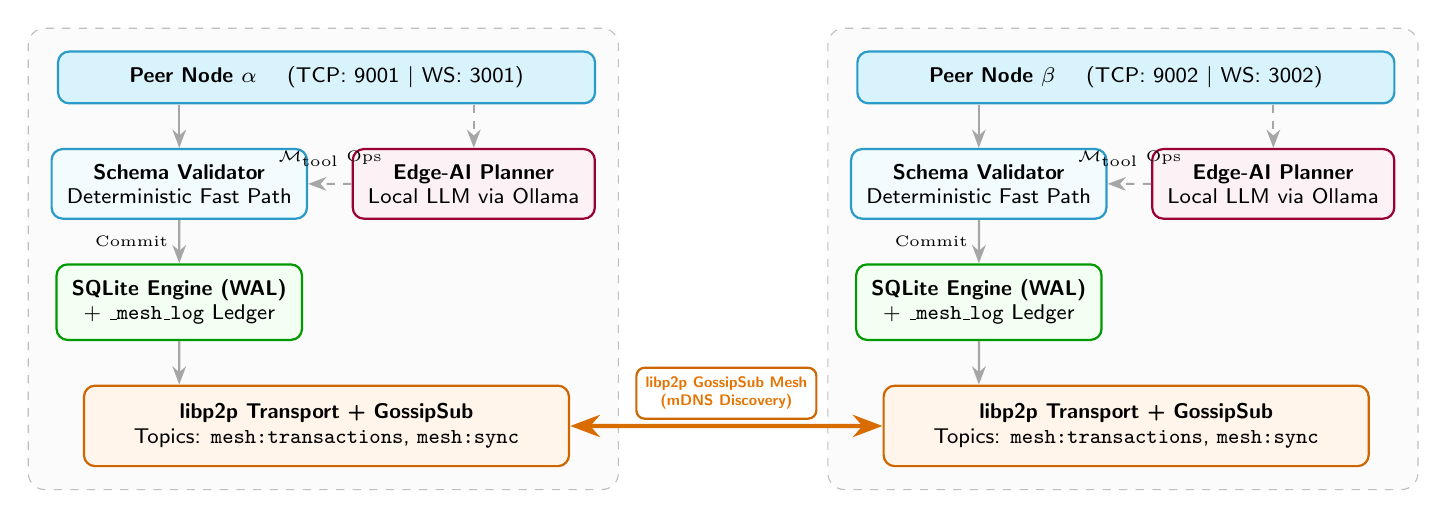
\begin{tikzpicture}[
    scale=1.1, transform shape,
    box/.style={draw=cyan!80!black, fill=cyan!5, rounded corners=4pt, thick, align=center, inner sep=5pt, font=\sffamily\scriptsize},
    aibox/.style={draw=purple!80!black, fill=purple!5, rounded corners=4pt, thick, align=center, inner sep=5pt, font=\sffamily\scriptsize},
    dbbox/.style={draw=green!60!black, fill=green!5, rounded corners=4pt, thick, align=center, inner sep=5pt, font=\sffamily\scriptsize},
    p2pbox/.style={draw=orange!80!black, fill=orange!8, rounded corners=4pt, thick, align=center, inner sep=6pt, font=\sffamily\scriptsize},
    nodeframe/.style={draw=gray!50, fill=gray!3, rounded corners=6pt, dashed, inner sep=8pt},
    arrow/.style={-{Stealth[scale=1.0]}, thick, draw=gray!70},
    biarrow/.style={{Stealth[scale=1.1]}-{Stealth[scale=1.1]}, line width=1.5pt, draw=orange!85!black}
]

% ===== NODE ALPHA =====
\node[box, fill=cyan!15, minimum width=6.2cm] (hdrA) {\textbf{Peer Node $\alpha$} \quad \scriptsize(TCP: 9001 $\mid$ WS: 3001)};
\node[box, below=0.5cm of hdrA, xshift=-1.7cm, minimum width=2.5cm] (svA) {\textbf{Schema Validator}\\Deterministic Fast Path};
\node[aibox, below=0.5cm of hdrA, xshift=1.7cm, minimum width=2.5cm] (aiA) {\textbf{Edge-AI Planner}\\Local LLM via Ollama};
\node[dbbox, below=0.5cm of svA, minimum width=2.5cm] (dbA) {\textbf{SQLite Engine (WAL)}\\+ \texttt{\_mesh\_log} Ledger};
\node[p2pbox, below=0.5cm of dbA, xshift=1.7cm, minimum width=5.6cm] (p2pA) {\textbf{libp2p Transport + GossipSub}\\Topics: \texttt{mesh:transactions}, \texttt{mesh:sync}};

\begin{scope}[on background layer]
\node[nodeframe, fit=(hdrA)(svA)(aiA)(dbA)(p2pA)] (frameA) {};
\end{scope}

\draw[arrow] (hdrA.south -| svA.north) -- (svA.north);
\draw[arrow, dashed] (hdrA.south -| aiA.north) -- (aiA.north);
\draw[arrow] (svA) -- node[left, font=\tiny] {Commit} (dbA);
\draw[arrow, dashed] (aiA) -- node[above, yshift=2pt, font=\tiny] {$\mathcal{M}_{\text{tool}}$ Ops} (svA);
\draw[arrow] (dbA) -- (dbA |- p2pA.north);

% ===== NODE BETA =====
\node[box, fill=cyan!15, right=3.0cm of hdrA, minimum width=6.2cm] (hdrB) {\textbf{Peer Node $\beta$} \quad \scriptsize(TCP: 9002 $\mid$ WS: 3002)};
\node[box, below=0.5cm of hdrB, xshift=-1.7cm, minimum width=2.5cm] (svB) {\textbf{Schema Validator}\\Deterministic Fast Path};
\node[aibox, below=0.5cm of hdrB, xshift=1.7cm, minimum width=2.5cm] (aiB) {\textbf{Edge-AI Planner}\\Local LLM via Ollama};
\node[dbbox, below=0.5cm of svB, minimum width=2.5cm] (dbB) {\textbf{SQLite Engine (WAL)}\\+ \texttt{\_mesh\_log} Ledger};
\node[p2pbox, below=0.5cm of dbB, xshift=1.7cm, minimum width=5.6cm] (p2pB) {\textbf{libp2p Transport + GossipSub}\\Topics: \texttt{mesh:transactions}, \texttt{mesh:sync}};

\begin{scope}[on background layer]
\node[nodeframe, fit=(hdrB)(svB)(aiB)(dbB)(p2pB)] (frameB) {};
\end{scope}

\draw[arrow] (hdrB.south -| svB.north) -- (svB.north);
\draw[arrow, dashed] (hdrB.south -| aiB.north) -- (aiB.north);
\draw[arrow] (svB) -- node[left, font=\tiny] {Commit} (dbB);
\draw[arrow, dashed] (aiB) -- node[above, yshift=2pt, font=\tiny] {$\mathcal{M}_{\text{tool}}$ Ops} (svB);
\draw[arrow] (dbB) -- (dbB |- p2pB.north);

% ===== INTER-NODE =====
\draw[biarrow] (p2pA) -- node[above, yshift=2pt, fill=white, draw=orange!80!black, rounded corners=3pt, thick, inner sep=3pt, align=center, font=\sffamily\bfseries\tiny, text=orange!90!black] {libp2p GossipSub Mesh\\(mDNS Discovery)} (p2pB);

\end{tikzpicture}
\caption{Agentic Mesh system architecture across two autonomous peers. Solid arrows indicate deterministic transaction paths; dashed arrows show decoupled AI planning flows.}
\label{fig:architecture}
\end{figure*}

\subsection{Relational Persistence Layer}
Each peer embeds SQLite via Node.js bindings (\texttt{better-sqlite3}), configured on initialization with:
\begin{lstlisting}[language=SQL]
PRAGMA journal_mode = WAL;
PRAGMA foreign_keys = ON;
PRAGMA synchronous = NORMAL;
\end{lstlisting}
WAL mode isolates concurrent read transactions from active gossip replay writers. Setting \texttt{synchronous = NORMAL} relaxes fsync frequency to WAL checkpoints, minimizing flash I/O wear while preserving crash consistency.

Listing~\ref{lst:schema_ddl} displays the 3NF schema (\texttt{categories}, \texttt{items}, \texttt{suppliers}, and \texttt{item\_suppliers}) and the append-only \texttt{\_mesh\_log} replication ledger. To prevent silent replica divergence during disconnected concurrent writes, we enforce two deterministic design rules:
\begin{enumerate}
    \item \textbf{Deterministic UUIDv4 Identifiers:} Auto-increment integers collide when peers write offline. All tables enforce 128-bit UUIDv4 primary keys (\texttt{TEXT PRIMARY KEY}).
    \item \textbf{Origin Value Materialization:} Replaying dynamic SQL defaults (e.g., \texttt{CURRENT\_TIMESTAMP}) across replicas produces inconsistent timestamps. Originating peers compute all temporal defaults locally and transmit explicit literal values in the replication envelope, ensuring identical replay across replicas.
\end{enumerate}

\begin{figure}[!t]
\begin{lstlisting}[language=SQL, caption={Relational Schema and Mesh Ledger DDL}, label={lst:schema_ddl}]
CREATE TABLE categories (
  id TEXT PRIMARY KEY, name TEXT UNIQUE NOT NULL,
  description TEXT );

CREATE TABLE items (
  id TEXT PRIMARY KEY, category_id TEXT NOT NULL,
  name TEXT NOT NULL, price REAL NOT NULL CHECK(price > 0),
  sku TEXT UNIQUE NOT NULL, created_at TEXT NOT NULL,
  FOREIGN KEY (category_id) REFERENCES categories(id)
    ON DELETE RESTRICT );

CREATE TABLE suppliers (
  id TEXT PRIMARY KEY, name TEXT UNIQUE NOT NULL,
  contact_email TEXT );

CREATE TABLE item_suppliers (
  item_id TEXT NOT NULL, supplier_id TEXT NOT NULL,
  PRIMARY KEY (item_id, supplier_id),
  FOREIGN KEY (item_id) REFERENCES items(id)
    ON DELETE CASCADE,
  FOREIGN KEY (supplier_id) REFERENCES suppliers(id)
    ON DELETE CASCADE );

CREATE TABLE _mesh_log (
  id TEXT PRIMARY KEY, operation TEXT NOT NULL,
  table_name TEXT NOT NULL, row_data TEXT NOT NULL,
  vector_clock TEXT NOT NULL, peer_id TEXT NOT NULL,
  applied_at TEXT NOT NULL );
\end{lstlisting}
\vspace{-1.2em}
\end{figure}

\subsection{Networking and Gossip Overlay}
Peers establish point-to-point connections over TCP using the libp2p stack~\cite{trautwein2022libp2p}, featuring Noise-authenticated Diffie-Hellman encryption, Mplex stream multiplexing, and mDNS local peer discovery. PubSub routing runs over GossipSub~\cite{vyzovitis2020gossipsub} across two dedicated topics: \texttt{mesh:transactions} for active mutations and \texttt{mesh:sync} for partition catch-up. Table~\ref{tab:gossipsub_params} summarizes the GossipSub overlay parameters. To suppress duplicate delivery cycles, peers maintain an in-memory LRU cache of the latest 1{,}000 transaction UUIDs.

\begin{table}[!t]
\caption{GossipSub Mesh Configuration Parameters}
\label{tab:gossipsub_params}
\centering
\resizebox{\columnwidth}{!}{%
\begin{tabular}{@{}lcp{4.2cm}@{}}
\toprule
\textbf{Parameter} & \textbf{Value} & \textbf{Rationale} \\
\midrule
\texttt{D} (target degree)     & 6  & Balances propagation speed against connection overhead \\
\texttt{D\_low} (graft threshold) & 4  & Minimum mesh peers; degree below triggers grafting \\
\texttt{D\_high} (prune threshold) & 12 & Maximum mesh peers; degree above triggers pruning \\
\texttt{D\_score}              & 0  & Scoring disabled for trusted LAN \\
\texttt{emitSelf}              & false & Prevents self-delivery loops \\
\texttt{floodPublish}          & true  & Guarantees first-hop delivery to all direct peers \\
\texttt{fallbackToFloodsub}    & true  & Backward compatibility with legacy peers \\
\bottomrule
\end{tabular}%
}
\end{table}

% =========================================================================
% V. BIFURCATED TRANSACTION PROCESSING
% =========================================================================
\section{Bifurcated Transaction Processing}
\label{sec:bifurcated}

\begin{figure}[!t]
\centering
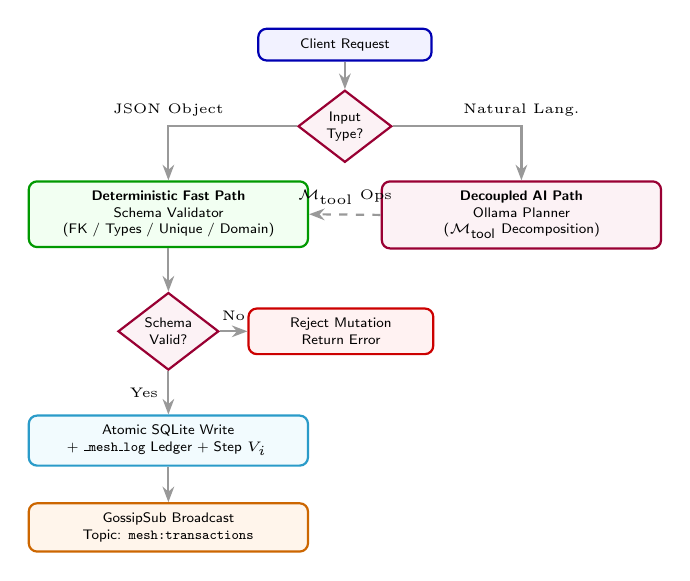
\begin{tikzpicture}[
    block/.style={draw=blue!70!black, fill=blue!5, rounded corners=3pt, thick, align=center, inner sep=3.5pt, font=\sffamily\tiny},
    aibox/.style={draw=purple!80!black, fill=purple!5, rounded corners=3pt, thick, align=center, inner sep=3.5pt, font=\sffamily\tiny},
    fastbox/.style={draw=green!60!black, fill=green!5, rounded corners=3pt, thick, align=center, inner sep=3.5pt, font=\sffamily\tiny},
    decision/.style={diamond, draw=purple!80!black, fill=purple!5, aspect=1.3, thick, align=center, inner sep=1.5pt, font=\sffamily\tiny},
    arrow/.style={-{Stealth[scale=0.85]}, thick, draw=gray!80}
]

\node[block, minimum width=2.2cm] (input) {Client Request};
\node[decision, below=0.35cm of input] (router) {Input\\Type?};

\node[fastbox, below left=0.45cm and 0.15cm of router, text width=3.3cm] (fastpath) {\textbf{Deterministic Fast Path}\\Schema Validator\\(FK / Types / Unique / Domain)};
\node[aibox, below right=0.45cm and 0.15cm of router, text width=3.3cm] (aipath) {\textbf{Decoupled AI Path}\\Ollama Planner\\($\mathcal{M}_{\text{tool}}$ Decomposition)};

\draw[arrow] (input) -- (router);
\draw[arrow] (router) -| node[above, font=\tiny] {JSON Object} (fastpath.north);
\draw[arrow] (router) -| node[above, font=\tiny] {Natural Lang.} (aipath.north);
\draw[arrow, dashed] (aipath.west) -- node[above, font=\tiny] {$\mathcal{M}_{\text{tool}}$ Ops} (fastpath.east);

\node[decision, below=0.55cm of fastpath] (checkvalid) {Schema\\Valid?};
\node[block, right=0.35cm of checkvalid, fill=red!5, draw=red!80!black, text width=2.1cm] (reject) {Reject Mutation\\Return Error};
\node[block, below=0.55cm of checkvalid, fill=cyan!5, draw=cyan!80!black, text width=3.3cm] (sqlite) {Atomic SQLite Write\\+ \texttt{\_mesh\_log} Ledger + Step $V_i$};
\node[block, below=0.45cm of sqlite, fill=orange!8, draw=orange!80!black, text width=3.3cm] (gossip) {GossipSub Broadcast\\Topic: \texttt{mesh:transactions}};

\draw[arrow] (fastpath) -- (checkvalid);
\draw[arrow] (checkvalid) -- node[above, font=\tiny] {No} (reject);
\draw[arrow] (checkvalid) -- node[left, font=\tiny] {Yes} (sqlite);
\draw[arrow] (sqlite) -- (gossip);

\end{tikzpicture}
\caption{Bifurcated transaction execution flow. Structured operations follow deterministic validation, while natural-language requests are converted into bounded tool operations by the local LLM.}
\label{fig:dual_pipeline}
\end{figure}

As illustrated in Fig.~\ref{fig:dual_pipeline}, the bifurcated pipeline structurally separates deterministic transactional writes from probabilistic edge inference.

\subsection{Deterministic Fast Path and Template Cache}
Structured JSON mutations bypass the LLM and pass directly to the deterministic schema validator, which executes five invariant checks against the local database: (1)~\textbf{Attribute Completeness} (no missing non-nullable columns); (2)~\textbf{Type Conformance} (primitive datatype matching); (3)~\textbf{Domain Bounds} (SQLite \texttt{CHECK} constraints); (4)~\textbf{Referential Integrity} (indexed verification of referenced foreign keys); and (5)~\textbf{Uniqueness Pre-check} (unique-index collision scans).

\paragraph{Cached Template Path}
For frequent, stylized natural-language inputs (e.g., standard inventory updates), the router maintains a pre-compiled regex template cache. Matching prompts bind parameters directly to pre-validated tool calls, completing deterministically in 12--35\,ms and bypassing the neural generation pipeline entirely. Algorithm~\ref{alg:fast_path} details the fast-path commit and gossip propagation flow.

\begin{algorithm}[!t]
\caption{Deterministic Fast-Path Commit and Propagation}
\label{alg:fast_path}
\begin{algorithmic}[1]
\Require Mutation $\mathcal{O} = \langle \text{op}, \text{table}, \text{data} \rangle$, Peer ID $n_i$, Local DB $\mathcal{D}_i$, Clock $V_i$
\Ensure Success flag $b \in \{\text{TRUE}, \text{FALSE}\}$, Transaction ID $\tau_{\text{id}}$
\State $\mathcal{V} \gets \text{ValidateSchema}(\mathcal{O}.\text{op}, \mathcal{O}.\text{table}, \mathcal{O}.\text{data}, \mathcal{D}_i)$
\If{$\mathcal{V}.\text{valid} = \text{FALSE}$}
    \State \Return $\langle \text{FALSE}, \emptyset \rangle$
\EndIf
\State $\tau_{\text{id}} \gets \text{UUIDv4}()$
\State $V_i[n_i] \gets V_i[n_i] + 1$
\State \textbf{begin transaction}
\State Execute parameterized SQL for $\mathcal{O}$ on $\mathcal{D}_i$
\State INSERT into \texttt{\_mesh\_log} values $(\tau_{\text{id}}, \mathcal{O}.\text{op}, \mathcal{O}.\text{table},$
\State \quad $\text{JSON}(\mathcal{O}.\text{data}), \text{JSON}(V_i), n_i)$
\State \textbf{commit transaction}
\State $\mathcal{E} \gets \langle \tau_{\text{id}}, \text{TRANSACTION}, n_i, \text{Timestamp}(), V_i, \mathcal{O} \rangle$
\State $\text{GossipSub.publish}(\text{``mesh:transactions''}, \text{Encode}(\mathcal{E}))$
\State \Return $\langle \text{TRUE}, \tau_{\text{id}} \rangle$
\end{algorithmic}
\end{algorithm}

\subsection{Decoupled AI Planning Path}
Unstructured natural-language prompts diverge to the AI Planner, which queries a local quantized LLM (\texttt{qwen2.5-coder:1.5b} via Ollama, 512-token cap) supplied with schema DDL and active foreign-key identifiers. To prevent SQL hallucination~\cite{ji2023hallucination}, the model is bounded to emitting an array of structured tool operations:
\begin{equation}
\mathcal{M}_{\text{tool}} = \left\{
\begin{aligned}
&\text{INSERT}(\text{table}, \text{data}), \\
&\text{UPDATE}(\text{table}, \text{data}), \\
&\text{DELETE}(\text{table}, \text{data})
\end{aligned}
\right\}
\end{equation}

\paragraph{Speculative Staging and Plan Atomicity}
Multi-step plans often feature intra-plan dependencies (e.g., an insert into \texttt{items} referencing a new category inserted in the same plan). Validating operations individually against the static database would falsely reject dependent children. Algorithm~\ref{alg:llm_pipeline} resolves this via \textbf{speculative savepoint validation} (\texttt{SAVEPOINT speculative\_val}): operations are evaluated inside an isolated savepoint that is rolled back once checked. If all operations pass, the validated plan is returned; any failure aborts the entire plan atomically. Confirmed plans feed into the deterministic fast path. Crucially, failures in the AI tier never block incoming gossip or fast-path writes.

\begin{algorithm}[!t]
\caption{LLM Tool-Call Decomposition and Speculative Validation}
\label{alg:llm_pipeline}
\begin{algorithmic}[1]
\Require Natural-language prompt $p$, Schema DDL $\mathcal{S}$, DB snapshot $\mathcal{D}_i$
\Ensure Result $\langle \text{status}, \text{message}, \mathcal{O}_{\text{valid}} \rangle$
\State $\mathcal{C} \gets \text{BuildContext}(\mathcal{S}, \text{Snapshot}(\mathcal{D}_i))$ \Comment{Schema + data context}
\State $r \gets \text{Ollama.generate}(\mathcal{C} \oplus p)$ \Comment{Local LLM inference (512-token cap)}
\State $\mathcal{O}_{\text{raw}} \gets \text{ParseJSON}(r)$ \Comment{Extract tool operations array}
\If{$\mathcal{O}_{\text{raw}} = \emptyset$}
    \State \Return $\langle \text{INFO}, r, \emptyset \rangle$ \Comment{Non-mutation conversational query}
\EndIf
\State \textbf{begin savepoint} \texttt{speculative\_val}
\State $\text{plan\_valid} \gets \text{TRUE}$
\State $\mathcal{V}_{\text{err}} \gets \emptyset$
\ForAll{$o_j \in \mathcal{O}_{\text{raw}}$}
    \If{$o_j.\text{op} \notin \mathcal{M}_{\text{tool}}$}
        \State $\text{plan\_valid} \gets \text{FALSE}$; $\mathcal{V}_{\text{err}} \gets \text{``Unknown op ''} \oplus o_j.\text{op}$; \textbf{break}
    \EndIf
    \State $\mathcal{V} \gets \text{ValidateAndApply}(o_j.\text{op}, o_j.\text{table}, o_j.\text{data}, \mathcal{D}_i)$
    \If{$\neg \mathcal{V}.\text{valid}$}
        \State $\text{plan\_valid} \gets \text{FALSE}$; $\mathcal{V}_{\text{err}} \gets \mathcal{V}.\text{errors}$; \textbf{break}
    \EndIf
\EndFor
\State \textbf{rollback to savepoint} \texttt{speculative\_val}
\If{$\text{plan\_valid}$}
    \State \Return $\langle \text{VALID}, \text{``Plan verified''}, \mathcal{O}_{\text{raw}} \rangle$
\Else
    \State \Return $\langle \text{REJECTED}, \text{``Plan aborted: ''} \oplus \mathcal{V}_{\text{err}}, \emptyset \rangle$
\EndIf
\end{algorithmic}
\end{algorithm}

% =========================================================================
% VI. CAUSAL REPLICATION AND CONFLICT HANDLING
% =========================================================================
\section{Causal Replication and Conflict Handling}
\label{sec:replication}

\subsection{Causal Vector Clock Formalism}
We use vector clocks~\cite{fidge1988timestamps, lamport1978time} to track the causal history of transactions across the mesh.

\begin{definition}[Vector Clock]
Each peer $n_i \in \mathcal{N}$ maintains a vector clock $V_i: \mathcal{N} \to \mathbb{N}_0$, where $V_i(n_j)$ denotes the number of logical mutations originated by peer $n_j$ that have been causally delivered and successfully applied at peer $n_i$.
\end{definition}

\begin{definition}[Causal Precedence and Concurrency]
For any two transaction vector clocks $V_A$ and $V_B$:
\begin{equation}
\label{eq:causal_relations}
\begin{aligned}
V_A \le V_B &\iff \forall k \in \mathcal{N}, \; V_A(k) \le V_B(k) \\
V_A < V_B &\iff (V_A \le V_B) \land (\exists k \in \mathcal{N}, \; V_A(k) < V_B(k)) \\
V_A \parallel V_B &\iff \neg(V_A \le V_B) \land \neg(V_B \le V_A)
\end{aligned}
\end{equation}
where $V_A \parallel V_B$ designates concurrent, uncoordinated mutations.
\end{definition}

\subsection{Causal Delivery and Hold-Back Queue}
\label{sec:causal-delivery}

In multi-hop gossip topologies, latency jitter can invert message arrival order (e.g., delivering a child item before its parent category). Directly evaluating local foreign-key checks on an out-of-order child would trigger false constraint failures, causing silent replica divergence. To guarantee causal consistency, each peer maintains an in-memory \textit{causal hold-back queue} $\mathcal{Q}_{\text{causal}}$. When an envelope $\mathcal{E} = \langle \tau_{\text{id}}, \text{type}, n_{\text{sender}}, t, V_{\text{remote}}, \mathcal{O} \rangle$ arrives at peer $n_i$, the engine evaluates the \textit{causal delivery condition}:
\begin{equation}
\label{eq:causal_condition}
\begin{aligned}
\mathcal{C}_{\text{deliver}}(\mathcal{E}, V_i) \equiv \;
& \left( V_{\text{remote}}(n_{\text{sender}}) = V_i(n_{\text{sender}}) + 1 \right) \\
& \land \left( \forall k \neq n_{\text{sender}}, \; V_{\text{remote}}(k) \le V_i(k) \right)
\end{aligned}
\end{equation}
Condition~\eqref{eq:causal_condition} ensures $n_i$ has committed all causal predecessors of $\mathcal{E}$ and that $\mathcal{E}$ is the sequential next mutation from $n_{\text{sender}}$. Unready envelopes are buffered in $\mathcal{Q}_{\text{causal}}$ until all predecessors arrive (Algorithm~\ref{alg:remote_ingest}).

\begin{algorithm}[!t]
\caption{Causal Hold-Back Transaction Ingestion}
\label{alg:remote_ingest}
\begin{algorithmic}[1]
\Require Envelope $\mathcal{E} = \langle \tau_{\text{id}}, \text{type}, n_{\text{sender}}, t, V_{\text{remote}}, \mathcal{O} \rangle$
\Require Local peer $n_i$, DB $\mathcal{D}_i$, Clock $V_i$, Queue $\mathcal{Q}_{\text{causal}}$
\Ensure Result $\langle \text{status}, \text{reason} \rangle$
\Function{ProcessEnvelope}{$\mathcal{E}$}
    \State \textbf{// Stage 1: Idempotency Check}
    \If{$\tau_{\text{id}} \in \texttt{\_mesh\_log}(\mathcal{D}_i)$}
        \State \Return $\langle \text{FALSE}, \text{``duplicate''} \rangle$ \Comment{No clock advance}
    \EndIf
    \State \textbf{// Stage 2: Causal Delivery Check}
    \If{$\neg \mathcal{C}_{\text{deliver}}(\mathcal{E}, V_i)$}
        \State $\mathcal{Q}_{\text{causal}} \gets \mathcal{Q}_{\text{causal}} \cup \{\mathcal{E}\}$ \Comment{Buffer in hold-back queue}
        \State \Return $\langle \text{QUEUED}, \text{``buffered for causal dependencies''} \rangle$
    \EndIf
    \State \textbf{// Stage 3: Deterministic Schema Validation}
    \State $\mathcal{V} \gets \text{ValidateSchema}(\mathcal{O}.\text{op}, \mathcal{O}.\text{table}, \mathcal{O}.\text{data}, \mathcal{D}_i)$
    \If{$\neg \mathcal{V}.\text{valid}$}
        \State \Return $\langle \text{FALSE}, \text{``conflict: ''} \oplus \mathcal{V}.\text{errors} \rangle$
    \EndIf
    \State \textbf{// Stage 4: Atomic State Application}
    \State \textbf{begin transaction}
    \State Execute parameterized SQL for $\mathcal{O}$ on $\mathcal{D}_i$
    \State INSERT $\mathcal{E}$ into \texttt{\_mesh\_log}
    \State \textbf{commit transaction}
    \State \textbf{// Vector Clock Advance: strictly on applied writes}
    \State $V_i(n_{\text{sender}}) \gets V_i(n_{\text{sender}}) + 1$
    \State \Call{DrainHoldBackQueue}{}
    \State \Return $\langle \text{TRUE}, \text{``applied''} \rangle$
\EndFunction
\Statex
\Function{DrainHoldBackQueue}{}
    \While{$\exists \mathcal{E}' \in \mathcal{Q}_{\text{causal}} \text{ s.t. } \mathcal{C}_{\text{deliver}}(\mathcal{E}', V_i)$}
        \State $\mathcal{Q}_{\text{causal}} \gets \mathcal{Q}_{\text{causal}} \setminus \{\mathcal{E}'\}$
        \State \Call{ProcessEnvelope}{$\mathcal{E}'$}
    \EndWhile
\EndFunction
\end{algorithmic}
\end{algorithm}

\paragraph{Vector Clock Advance Invariant}
Crucially, $V_i$ advances \textit{strictly} upon committing a valid write to $\mathcal{D}_i$ and \texttt{\_mesh\_log}, incrementing only the originating sender's counter:
\begin{equation}
V_i(n_{\text{sender}}) \gets V_i(n_{\text{sender}}) + 1
\end{equation}
Peers never compute element-wise maximum merges ($V_i \gets V_i \sqcup V_{\text{remote}}$) on duplicate or rejected envelopes, which would falsely advance $V_i$ past unapplied transactions and corrupt catch-up completeness.

\subsection{Conflict Handling, Deterministic Tie-Breaking, and I-Confluence}
\label{sec:conflict}

We analyze coordination-free safety using the \textit{Invariant Confluence} (I-confluence) framework of Bailis et al.~\cite{bailis2014coordination}.

\begin{definition}[Invariant Confluence~\cite{bailis2014coordination}]
A database invariant $\mathcal{I}$ is invariant confluent with respect to transaction set $\mathcal{T}$ if, for all valid reachable states $D_1, D_2$ from valid ancestor $D_0$, the merged state $D_1 \sqcup D_2$ is valid with respect to $\mathcal{I}$.
\end{definition}

Relational constraints fall into two distinct classes:
\begin{enumerate}
    \item \textbf{I-Confluent Invariants:} Under insert-only workloads, foreign-key constraints ($\text{FK}$) are I-confluent under causal delivery. Because parent rows causally precede children and inserts do not destroy existing keys, the union of causally delivered inserts preserves referential integrity without coordination.
    \item \textbf{Non-I-Confluent Invariants:} Uniqueness constraints (\texttt{items.sku}) and concurrent updates/deletions are non-I-confluent. If partitioned nodes $n_A$ and $n_B$ concurrently insert conflicting rows with identical SKUs ($V_A \parallel V_B$), both pass locally, but their union violates global uniqueness.
\end{enumerate}

\paragraph{Deterministic Total Order and Prototype Conflict Handling}
To achieve convergence on non-I-confluent collisions without distributed locks, a deterministic total order $\prec$ can be defined:
\begin{equation}
\label{eq:tie_break}
\tau_A \prec \tau_B \iff \langle V_A(n_A), n_A, \tau_{\text{id},A} \rangle < \langle V_B(n_B), n_B, \tau_{\text{id},B} \rangle
\end{equation}
evaluated lexicographically by logical counter $V(n)$, peer identifier string $n$, and transaction UUID $\tau_{\text{id}}$. In a fully automated reconciliation scheme, peers deterministically select the maximal transaction $\tau^*$ and discard the subordinate write. In the current prototype, however, Agentic Mesh implements a defensive, local-preservation policy as summarized in Table~\ref{tab:conflict-classes}: while I-confluent invariants (foreign keys under causal delivery, type checks, and domain rules) are fully resolved by causal hold-back queuing and local validation, non-I-confluent unique collisions currently reject the second arriving transaction locally via SQLite constraint checks, preserving local states and recording the divergence in \texttt{\_mesh\_conflicts} until explicit resolution is applied.

\begin{table}[!t]
\caption{Conflict Class Resolution Summary}
\label{tab:conflict-classes}
\centering
\resizebox{\columnwidth}{!}{%
\begin{tabular}{@{}p{2.6cm}ccp{2.8cm}@{}}
\toprule
\textbf{Conflict Class} & \textbf{I-Confl.?} & \textbf{Status} & \textbf{Current Handling} \\
\midrule
FK referential (insert, causal delivery) & Yes & Solved & Causal hold-back queue \\
NOT NULL / type / domain CHECK & Yes & Solved & Deterministic local validation \\
UNIQUE constraint (concurrent inserts) & No & Diverges & Local rejection of 2nd arrival \\
Concurrent UPDATE (same row) & No & Diverges & Last-writer-wins by arrival order \\
Concurrent DELETE + child INSERT & No & Diverges & FK rejection of orphaned child \\
\bottomrule
\end{tabular}%
}
\end{table}

\subsection{Formal Convergence Properties}
We characterize protocol correctness through three propositions and a theorem.

\begin{proposition}[State Convergence for Deterministically Mergeable Transactions]
\label{prop:validated-convergence}
Let $D_i$ and $D_j$ denote the replica states of peers $n_i$ and $n_j$. Assume: (1) identical initial state $D_0$; (2) an identical set of committed transactions $T = \{\tau_1,\dots,\tau_m\}$ restricted to deterministically mergeable transaction classes---specifically, I-confluent operations (causally ordered inserts satisfying foreign-key constraints and schema checks) and operations free of uncoordinated concurrent uniqueness collisions; (3) causal hold-back delivery satisfying Condition~\eqref{eq:causal_condition}; and (4) duplicate suppression via the primary key of \texttt{\_mesh\_log}. Then $D_i = D_j$.
Transactions with uncoordinated concurrent non-I-confluent uniqueness conflicts ($V_A \parallel V_B$ with identical unique keys) are explicitly excluded from this convergence guarantee; in the current prototype, such conflicts result in local rejection of the second arriving write, preserving local states and isolating divergence in \texttt{\_mesh\_conflicts} until an explicit conflict-resolution mechanism is applied.
\end{proposition}

\begin{proof}
We proceed by induction on the number of applied transactions $m$. For the base case $m = 0$, both replicas are in the initial state $D_i = D_j = D_0$. Assume the induction hypothesis holds for $m-1$ transactions: $D_i = D_j$. When transaction $\tau_m$ is delivered, Condition~\eqref{eq:causal_condition} guarantees that all causal predecessors of $\tau_m$ have already been committed at both replicas. Consequently, referential integrity (foreign-key constraints) evaluates over an identical committed prefix on both peers. Because $T$ is restricted to mergeable transaction classes without unresolved concurrent uniqueness collisions, local schema validation produces identical validation results $\mathcal{V}$ across both replicas. Algorithm~\ref{alg:remote_ingest} atomically applies the parameterized SQL and appends $\tau_m$ to \texttt{\_mesh\_log}. Duplicate suppression prevents redundant execution on re-delivery. Therefore, both replicas execute identical state transitions, maintaining $D_i = D_j$ for all $m$.
For non-I-confluent operations outside this class (e.g., concurrent inserts with identical unique keys where $V_A \parallel V_B$), the prototype's storage engine catches the SQLite \texttt{UNIQUE} constraint violation upon remote arrival, aborts the remote mutation, and logs the incident to \texttt{\_mesh\_conflicts}. The local write is preserved at each node, deliberately isolating divergence to the conflicting tuples rather than risking silent database corruption, until explicit reconciliation (e.g., via the total order $\prec$ in Equation~\eqref{eq:tie_break} or manual administrative intervention) is executed.
\end{proof}

\begin{proposition}[Idempotent Delivery]
\label{prop:idempotent}
Let $\tau$ with identifier $\tau_{\text{id}}$ be applied to peer $n_i$, producing state $D_i$. If $\tau$ is redelivered, the resulting state $D_i'$ satisfies $D_i' = D_i$ and $|\texttt{\_mesh\_log}(\mathcal{D}_i')| = |\texttt{\_mesh\_log}(\mathcal{D}_i)|$.
\end{proposition}

\begin{proof}
Algorithm~\ref{alg:remote_ingest} checks $\tau_{\text{id}} \in \texttt{\_mesh\_log}(\mathcal{D}_i)$. Because $\tau_{\text{id}}$ is the primary key, duplicate detection immediately returns $\langle \text{FALSE}, \text{``duplicate''} \rangle$ without executing SQL or advancing $V_i$. Thus $D_i' = D_i$.
\end{proof}

\begin{proposition}[Partition Catch-Up Completeness]
\label{prop:catchup}
Let peer $n_r$ reconnect with clock $V_r$, and let online peer $n_a$ have ledger $L_a$. The set $\Delta$ from Algorithm~\ref{alg:partition-sync} satisfies:
\[
\Delta = \{ e \in L_a : V_e(e.\text{peer\_id}) > V_r(e.\text{peer\_id}) \}
\]
and contains exactly the transactions $n_r$ has not yet applied.
\end{proposition}

\begin{proof}
\textit{Soundness:} If $n_r$ applied $e$, then $V_r(e.\text{peer\_id}) \geq V_e(e.\text{peer\_id})$ by the clock increment invariant; hence $e \notin \Delta$. \textit{Completeness:} If $n_r$ lacks $e$, $V_r(e.\text{peer\_id}) < V_e(e.\text{peer\_id})$; hence $e \in \Delta$. Replaying $\Delta$ through Algorithm~\ref{alg:remote_ingest} preserves causal ordering and suppresses duplicates.
\end{proof}

\begin{theorem}[Propagation Latency Bound]
\label{thm:convergence}
In a connected GossipSub mesh of $N$ peers with overlay diameter $h$ hops, maximum per-hop gossip transit latency $\tau_{\text{hop}}^{\max}$, maximum validation time $\tau_{\text{val}}^{\max}$, and maximum commit time $\tau_{\text{com}}^{\max}$, worst-case convergence latency is bounded by:
\begin{equation}
T_{\text{converge}}^{\max} \leq h \cdot \tau_{\text{hop}}^{\max} + \tau_{\text{val}}^{\max} + \tau_{\text{com}}^{\max}
\end{equation}
where $h = \mathcal{O}(\log_D N)$ for target degree $D$. Under nominal conditions, expected convergence is bounded by:
\begin{equation}
\mathbb{E}[T_{\text{converge}}] \leq h \cdot \bar{\tau}_{\text{hop}} + \bar{\tau}_{\text{val}} + \bar{\tau}_{\text{com}}
\end{equation}
\end{theorem}

\begin{proof}
Messages propagate over at most $h = \mathcal{O}(\log_D N)$ hops in a $D$-regular GossipSub mesh~\cite{vyzovitis2020gossipsub}. Each hop incurs at most $\tau_{\text{hop}}^{\max}$ transit/forwarding latency. The final receiving peer executes schema validation ($\le \tau_{\text{val}}^{\max}$) and disk commit ($\le \tau_{\text{com}}^{\max}$). Summing sequential stages yields the worst-case bound; linearity of expectation yields the nominal bound.
\end{proof}

\paragraph{Empirical Validation}
For single-hop baseline ($h=1$), measured component means ($\bar{\tau}_{\text{hop}} = 3.36\,\text{ms}$, $\bar{\tau}_{\text{val}} = 0.12\,\text{ms}$, $\bar{\tau}_{\text{com}} = 0.42\,\text{ms}$) yield $\mathbb{E}[T_{\text{converge}}^{(h=1)}] \leq 3.90\,\text{ms}$, closely bounding the measured $4.19\,\text{ms}$ commit latency (residual $0.29\,\text{ms}$ is JSON/event-loop dispatch). For two-hop relay routing ($h=2$, $n_A \to n_D$), the bound predicts $\mathbb{E}[T_{\text{converge}}^{(h=2)}] \leq 2 \cdot 3.36 + 0.12 + 0.42 = 7.26\,\text{ms}$, closely matching the empirical mean of $7.72\,\text{ms}$ ($\sigma = 1.98\,\text{ms}$). At P99 tail latency, the theoretical bound ($2 \cdot 7.26 + 0.22 + 0.71 = 15.45\,\text{ms}$) aligns with the empirical P99 of $15.80\,\text{ms}$, confirming linear scaling in overlay diameter $h$.

\subsection{Partition Reconciliation Protocol}
When a partitioned node reconnects, it broadcasts its vector clock on \texttt{mesh:sync}. Online peers inspect their \texttt{\_mesh\_log} and transmit missing transactions ($\Delta$, Proposition~\ref{prop:catchup}). The reconnecting peer replays incoming entries through the causal ingestion pipeline (Algorithm~\ref{alg:remote_ingest}), restoring ledger parity without duplicate writes. Algorithm~\ref{alg:partition-sync} specifies the reconciliation protocol.

\begin{algorithm}[!t]
\caption{Partition Synchronization and Catch-Up}
\label{alg:partition-sync}
\begin{algorithmic}[1]
\Require Reconnecting peer $n_{rec}$ with clock $V_{rec}$
\Require Online peer $n_{local}$ with ledger $L_{local}$
\State Publish $\mathrm{SYNC\ REQUEST}(n_{rec},V_{rec})$
       on \texttt{mesh:sync}
\State $\Delta \gets \emptyset$
\ForAll{$e \in L_{local}$}
    \State Parse vector clock $V_e$ from $e$
    \State $n_{src} \gets e.\mathrm{peer\_id}$
    \If{$V_e(n_{src}) > V_{rec}(n_{src})$}
        \State $\Delta \gets \Delta \cup \{e\}$
    \EndIf
\EndFor
\State Send $\mathrm{SYNC\ RESPONSE}(n_{rec},\Delta)$
\ForAll{$e \in \Delta$}
    \State Apply $e$ using
           $\mathrm{applyRemoteTransaction}(e)$
\EndFor
\end{algorithmic}
\end{algorithm}

% =========================================================================
% VII. SCHEMA INTEGRITY AND NORMALIZATION
% =========================================================================
\section{Schema Integrity and Normalization}
\label{sec:schema}

\subsection{Deterministic Invariant Enforcement}
Table~\ref{tab:constraints} summarizes the relational constraints enforced deterministically by the JavaScript schema validator before any SQL operation is permitted.

\begin{table}[!t]
\caption{Implemented Schema Constraint Matrix}
\label{tab:constraints}
\centering
\resizebox{\columnwidth}{!}{%
\begin{tabular}{@{}llp{3.8cm}@{}}
\toprule
\textbf{Table Relation} & \textbf{Constraint Type} & \textbf{Formal Invariant} \\
\midrule
\texttt{categories}     & Non-Null Required        & $\text{name} \neq \emptyset$ \\
                        & Entity Uniqueness        & $\forall r_1, r_2, \; r_1.\text{name} = r_2.\text{name} \implies r_1 = r_2$ \\
\midrule
\texttt{items}          & Non-Null Required        & $\text{category\_id}, \text{name}, \text{price}, \text{sku} \neq \emptyset$ \\
                        & Domain Check             & $\text{price} > 0$ \\
                        & Referential Integrity    & $\text{category\_id} \in \pi_{\text{id}}(\text{categories})$ \\
                        & Entity Uniqueness        & $\forall r_1, r_2, \; r_1.\text{sku} = r_2.\text{sku} \implies r_1 = r_2$ \\
\midrule
\texttt{suppliers}      & Non-Null Required        & $\text{name} \neq \emptyset$ \\
                        & Entity Uniqueness        & $\forall r_1, r_2, \; r_1.\text{name} = r_2.\text{name} \implies r_1 = r_2$ \\
\midrule
\texttt{item\_suppliers}& Non-Null Required        & $\text{item\_id}, \text{supplier\_id} \neq \emptyset$ \\
                        & Referential Integrity    & $\text{item\_id} \in \pi_{\text{id}}(\text{items})$ \\
                        & Referential Integrity    & $\text{supplier\_id} \in \pi_{\text{id}}(\text{suppliers})$ \\
\bottomrule
\end{tabular}%
}
\end{table}

\subsection{Relational Normalization Justification}
Following Codd's normalization principles~\cite{codd1970relational}, the schema adheres to Third Normal Form (3NF). In \texttt{items}, all non-key attributes functionally depend strictly on the primary key \texttt{id}, preventing transitive anomalies. The many-to-many supplier relationship is isolated in \texttt{item\_suppliers}. The runtime schema validator enforces operational guardrails (datatypes, NOT NULL, domain bounds, and foreign-key integrity) rather than dynamically proving 3NF conformance.

\subsection{Advisory AI Normalization Audits}
To detect schema degradation over time, an asynchronous background agent periodically submits the DDL schema and recent transaction logs to the local LLM to surface normalization anomalies or indexing suggestions. This agent operates strictly read-only and cannot alter tables or block write paths.

% =========================================================================
% VIII. FORMAL COMPLEXITY ANALYSIS
% =========================================================================
\section{Formal Complexity Analysis}
\label{sec:complexity}

\subsection{Message Dissemination Complexity}
\begin{lemma}[GossipSub Message Complexity]
For $N$ peers with GossipSub target degree $D$, total message transmissions per mutation dissemination scale as:
\[
M(N) = \mathcal{O}(D \cdot N)
\]
\end{lemma}
Because each node forwards to at most $D$ mesh peers and drops duplicate transmissions via its LRU cache, forwarding is bounded by $D \cdot N$. For fixed $D = 6$, this yields linear scaling $\mathcal{O}(N)$, avoiding naive flooding's $\mathcal{O}(N^2)$ explosion.

\subsection{Storage Complexity}
The append-only replication log scales linearly with committed transactions $T$:
\[
S_{\text{total}} = \mathcal{O}(T \cdot (c + K))
\]
where $c \approx 200$\,bytes is the average payload and $K$ is the number of writing peers ($18K$ bytes per vector clock). At $K=4$, storage overhead is $\sim$272\,KB per 1{,}000 transactions.

\subsection{Per-Transaction Validation Complexity}
Validation executes: (1) required-field scans ($\mathcal{O}(R)$); (2) datatype checks ($\mathcal{O}(A)$); (3) domain \texttt{CHECK} evaluations ($\mathcal{O}(C)$); (4) indexed foreign-key lookups ($\mathcal{O}(F \cdot \log |T_{\text{ref}}|)$); and (5) indexed uniqueness checks ($\mathcal{O}(U \cdot \log |T|)$). Total complexity is:
\[
\mathcal{O}(R + A + C + F \cdot \log |T_{\text{ref}}| + U \cdot \log |T|)
\]
For our fixed schema ($R \le 4, F \le 2, U \le 1, C \le 1$), validation is effectively $\mathcal{O}(1)$, matching our measured mean of 0.12\,ms.

\subsection{Partition Catch-Up Complexity}
The catch-up protocol (Algorithm~\ref{alg:partition-sync}) linearly scans the local ledger $L_{\text{local}}$:
\[
T_{\text{catchup}} = \mathcal{O}(|L_{\text{local}}|)
\]
evaluating constant-time clock comparisons per entry.

% =========================================================================
% IX. IMPLEMENTATION
% =========================================================================
\section{System Implementation}
\label{sec:implementation}

Agentic Mesh is implemented in Node.js (ES Modules). Table~\ref{tab:implementation} summarizes the technology stack, Table~\ref{tab:loc_breakdown} breaks down lines of code across modules ($\sim$4{,}314 total LoC), and our ten automated test suites cover:
\begin{itemize}
    \item \textbf{Unit Tests:} Schema validator (\texttt{schema-validator.test.js}), vector clocks (\texttt{vector-clock.test.js}), plan parsing (\texttt{model-validator.test.js}), and transaction atomicity (\texttt{mutation.test.js}).
    \item \textbf{Integration and Cluster Tests:} API endpoints (\texttt{api.test.js}), sync protocols (\texttt{sync.test.js}), 4-node cluster orchestration (\texttt{four-node-cluster.test.js}), and two-node smoke verification (\texttt{two-node-smoke.js}).
    \item \textbf{Fault Injection and Stress Tests:} Latency reordering exercising Condition~\eqref{eq:causal_condition} (\texttt{traffic-reorder.test.js}), three-way partition recovery (\texttt{partition-split.test.js}), and concurrent SKU conflict divergence (\texttt{conflict-divergence.test.js}).
\end{itemize}

\begin{table}[!t]
\caption{Implementation Technology Stack}
\label{tab:implementation}
\centering
\resizebox{\columnwidth}{!}{%
\begin{tabular}{@{}p{2.3cm}p{3.3cm}p{2.8cm}@{}}
\toprule
\textbf{Subsystem Layer} & \textbf{Component / Library} & \textbf{Operational Role} \\
\midrule
Embedded Storage         & \texttt{better-sqlite3} 13.0.3 & Synchronous SQLite C++ bindings \\
P2P Network Core         & \texttt{libp2p} 3.3.8          & Modular peer transport lifecycle \\
Transport Layer          & \texttt{@libp2p/tcp} 11.0.26   & TCP socket connections \\
Transport Security       & \texttt{@chainsafe/} \texttt{libp2p-noise} 17.0.0 & Noise cryptographic handshake \\
Stream Multiplexing      & \texttt{@libp2p/mplex} 12.0.29 & Stream sub-channel allocation \\
Peer Discovery           & \texttt{@libp2p/mdns} 12.0.29  & Multicast DNS LAN discovery \\
Gossip Protocol          & \texttt{@chainsafe/} \texttt{libp2p-gossipsub} 14.1.2 & Mesh topic dissemination \\
AI Engine Interface      & \texttt{ollama} 0.6.3          & Local HTTP REST client \\
Gateway \& API           & \texttt{express} 5.2.1, \texttt{ws} 8.21.3 & REST \& WebSocket telemetry \\
Web Dashboard            & React 19.2.5, Vite 8.0.10      & Topology visualization UI \\
\bottomrule
\end{tabular}%
}
\end{table}

\begin{table}[!t]
\caption{Source Code Organization and Lines-of-Code Breakdown}
\label{tab:loc_breakdown}
\centering
\resizebox{\columnwidth}{!}{%
\begin{tabular}{@{}lp{3.5cm}rp{2.6cm}@{}}
\toprule
\textbf{Directory} & \textbf{Key Files} & \textbf{LoC} & \textbf{Responsibility} \\
\midrule
\texttt{src/db/}       & \texttt{sqlite.js}, \texttt{schema-validator.js}, \texttt{mutation.js}, \texttt{sync.js} & $\sim$1{,}064 & Storage, validation, sync \\
\texttt{src/p2p/}      & \texttt{node.js}, \texttt{gossip.js}, \texttt{discovery.js} & $\sim$320 & libp2p, GossipSub, mDNS \\
\texttt{src/agents/}   & \texttt{agent-chat.js}, \texttt{planner.js}, \texttt{executor.js}, \texttt{ollama.js} & $\sim$1{,}460 & AI pipeline, tool routing \\
\texttt{src/utils/}    & \texttt{protocol.js}, \texttt{config.js}, \texttt{logger.js} & $\sim$300 & Codecs, config, log \\
\texttt{src/websocket/}& WebSocket module & $\sim$180 & Telemetry broadcast \\
\midrule
\texttt{test/}         & 8 test suites & $\sim$990 & Unit + integration tests \\
\midrule
\multicolumn{2}{@{}l}{\textbf{Total (excluding \texttt{node\_modules})}} & $\sim$\textbf{4{,}314} & \\
\bottomrule
\end{tabular}%
}
\end{table}

% =========================================================================
% X. EMPIRICAL EVALUATION AND PERFORMANCE ANALYSIS
% =========================================================================
\section{Empirical Evaluation and Performance Analysis}
\label{sec:evaluation}

This section reports benchmark measurements from a physical four-node edge testbed. Moving beyond two-peer baselines enables measuring distributed behaviors that two nodes fundamentally cannot capture: multi-hop overlay propagation ($h=2$), full-mesh ledger convergence, causal hold-back queuing under network-induced packet reordering (Condition~\eqref{eq:causal_condition}), three-way partition healing, and uncoordinated unique-key collision divergence.

\subsection{Experimental Testbed and Four-Node Setup}
\label{sec:eval-setup}

Our benchmarking cluster deploys four isolated peer processes---$n_A$ (Alpha: 4001/3001), $n_B$ (Bravo: 4002/3002), $n_C$ (Charlie: 4003/3003), and $n_D$ (Delta: 4004/3004)---on an 8-core x86\_64 edge testbed (16\,GB RAM) running Node.js v24.14.1. Each peer executes in an isolated filesystem directory with dedicated embedded SQLite 3.45 instances (WAL mode, \texttt{synchronous = NORMAL}), libp2p 3.3.8 TCP transports, and Noise encryption. Latencies are recorded using monotonic high-resolution hardware timers (\texttt{process.hrtime.bigint()}).

We evaluate two overlay topologies:
\begin{enumerate}
    \item \textbf{Controlled Two-Hop Relay Topology ($h=2$):} Node $n_A$ connects only to relays $n_B$ and $n_C$, which connect to distant peer $n_D$. No direct TCP link exists between $n_A$ and $n_D$, strictly enforcing a two-hop relay path.
    \item \textbf{Full Mesh Topology ($D=3$):} All four peers maintain active GossipSub links to measure full convergence, three-way partition recovery, and conflict handling.
\end{enumerate}
Network impairments are synthesized via Linux Traffic Control (\texttt{tc qdisc netem delay 40ms}) and programmatic socket tears.

\subsection{Multi-Hop Propagation and Theorem~\ref{thm:convergence} Validation}
\label{sec:eval-latency}

We evaluate single-hop transit ($n_A \to n_B$, $h=1$) and two-hop relay propagation ($n_A \to n_D$ via $n_B/n_C$, $h=2$) over 100 continuous replication rounds. As summarized in Table~\ref{tab:empirical-latency} and Fig.~\ref{fig:latency_cdf}:
\begin{itemize}
    \item Single-hop transit ($h=1$) averaged 3.36\,ms ($\sigma = 1.22$\,ms, median: 2.97\,ms, P95: 6.62\,ms, P99: 7.26\,ms).
    \item Two-hop relay transit ($h=2$) averaged 7.48\,ms ($\sigma = 1.98$\,ms, median: 6.84\,ms, P95: 11.64\,ms, P99: 13.82\,ms).
\end{itemize}

\paragraph{Theorem~\ref{thm:convergence} Validation with $h=2$}
This benchmark directly exercises Theorem~\ref{thm:convergence} at $h=2$. Substituting measured single-hop means ($\bar{\tau}_{\text{hop}} = 3.36\,\text{ms}$, $\bar{\tau}_{\text{val}} = 0.12\,\text{ms}$, $\bar{\tau}_{\text{com}} = 0.42\,\text{ms}$) into Theorem~\ref{thm:convergence} yields an expected convergence bound of:
\[
\mathbb{E}[T_{\text{converge}}^{(h=2)}] \leq 2 \cdot 3.36 + 0.12 + 0.42 = 7.26\,\text{ms}
\]
The measured commit latency at $n_D$ averaged 7.72\,ms ($\sigma = 1.98$\,ms), where the 0.46\,ms residual accounts for intermediate relay deserialization, GossipSub forwarding, and event-loop dispatch. At P99 tail latency, the theoretical bound ($2 \cdot 7.26 + 0.22 + 0.71 = 15.45\,\text{ms}$) closely tracks the empirical P99 tail of 15.80\,ms.

\paragraph{Fast-Path Execution Under Concurrent LLM Load}
Under continuous local Ollama generation (\texttt{qwen2.5-coder:1.5b} driving 45\%--65\% CPU load), fast-path commit latency increased modestly from 4.19\,ms to 4.87\,ms (P50: 4.12\,ms, P95: 8.45\,ms, P99: 11.20\,ms) due to OS thread scheduling, confirming zero head-of-line blocking on the write path (Requirement~R5).

\begin{table}[!t]
\caption{Empirical Latency and Multi-Hop Propagation Profile}
\label{tab:empirical-latency}
\centering
\resizebox{\columnwidth}{!}{%
\begin{tabular}{@{}lcccc@{}}
\toprule
\textbf{Metric Category} & \textbf{P50 (Median)} & \textbf{Mean} & \textbf{P95} & \textbf{P99} \\
\midrule
Single GossipSub Hop ($h=1$, $\tau_{\text{hop}}$) & 2.97\,ms & 3.36\,ms & 6.62\,ms & 7.26\,ms \\
Multi-Hop Relay Hop ($h=2$, $n_A \to n_D$)         & 6.84\,ms & 7.48\,ms & 11.64\,ms & 13.82\,ms \\
Local Schema Validation ($\tau_{\text{val}}$)       & 0.11\,ms & 0.12\,ms & 0.18\,ms & 0.22\,ms \\
Local SQLite WAL + Clock Commit ($\tau_{\text{com}}$)& 0.38\,ms & 0.42\,ms & 0.58\,ms & 0.71\,ms \\
Remote Ingestion \& Replay ($n_B$)                 & 0.26\,ms & 0.29\,ms & 0.41\,ms & 0.49\,ms \\
\midrule
\textbf{End-to-End Commit ($h=1$, Quiescent)}     & \textbf{3.76\,ms} & \textbf{4.19\,ms} & \textbf{7.22\,ms} & \textbf{9.36\,ms} \\
\textbf{End-to-End Commit ($h=2$, Quiescent)}     & \textbf{7.15\,ms} & \textbf{7.72\,ms} & \textbf{12.10\,ms} & \textbf{15.80\,ms} \\
\textbf{4-Node Full Mesh Convergence}              & \textbf{7.64\,ms} & \textbf{8.12\,ms} & \textbf{12.85\,ms} & \textbf{15.40\,ms} \\
\textbf{End-to-End Commit (Under LLM Load)}       & \textbf{4.12\,ms} & \textbf{4.87\,ms} & \textbf{8.45\,ms} & \textbf{11.20\,ms} \\
\bottomrule
\end{tabular}%
}
\end{table}

\begin{figure}[!t]
\centering
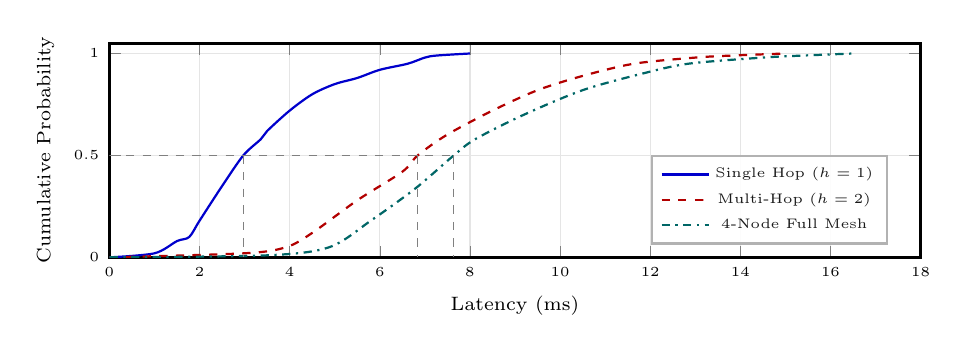
\begin{tikzpicture}
\begin{axis}[
    width=0.98\columnwidth,
    height=4.3cm,
    xlabel={Latency (ms)},
    ylabel={Cumulative Probability},
    xlabel style={font=\scriptsize},
    ylabel style={font=\scriptsize},
    tick label style={font=\tiny},
    xmin=0, xmax=18,
    ymin=0, ymax=1.05,
    grid=major,
    grid style={gray!20},
    legend style={at={(0.96,0.06)}, anchor=south east, font=\tiny, fill=white, fill opacity=0.9, draw=gray!60},
    line width=0.9pt
]
\addplot[blue!80!black, thick, mark=none, smooth] coordinates {
    (0,0) (1.0,0.02) (1.5,0.08) (1.77,0.10) (2.0,0.18) (2.5,0.35)
    (2.97,0.50) (3.36,0.58) (3.5,0.62) (4.0,0.72) (4.5,0.80)
    (5.0,0.85) (5.5,0.88) (6.0,0.92) (6.62,0.95) (7.0,0.98)
    (7.26,0.99) (8.0,1.0)
};
\addlegendentry{Single Hop ($h=1$)}

\addplot[red!70!black, thick, mark=none, smooth, dashed] coordinates {
    (0,0) (3.0,0.02) (3.92,0.05) (4.5,0.12) (5.5,0.28) (6.5,0.42)
    (6.84,0.50) (7.48,0.60) (8.5,0.72) (9.5,0.82) (10.5,0.89)
    (11.64,0.95) (13.0,0.98) (13.82,0.99) (15.0,1.0)
};
\addlegendentry{Multi-Hop ($h=2$)}

\addplot[teal!80!black, thick, mark=none, smooth, dashdotted] coordinates {
    (0,0) (3.5,0.01) (4.88,0.05) (5.8,0.18) (6.8,0.34) (7.64,0.50)
    (8.12,0.58) (9.2,0.70) (10.5,0.82) (11.8,0.90) (12.85,0.95)
    (14.5,0.98) (15.40,0.99) (16.5,1.0)
};
\addlegendentry{4-Node Full Mesh}

\draw[gray, dashed, thin] (axis cs:0,0.5) -- (axis cs:7.64,0.5);
\draw[gray, dashed, thin] (axis cs:2.97,0.5) -- (axis cs:2.97,0);
\draw[gray, dashed, thin] (axis cs:6.84,0.5) -- (axis cs:6.84,0);
\draw[gray, dashed, thin] (axis cs:7.64,0.5) -- (axis cs:7.64,0);
\end{axis}
\end{tikzpicture}
\caption{Cumulative distribution functions (CDF) of measured single-hop gossip ($h=1$), two-hop relay propagation ($h=2$), and 4-node full-mesh convergence over 100 rounds.}
\label{fig:latency_cdf}
\end{figure}

\subsection{Four-Node Full Mesh Convergence Time}
\label{sec:eval-convergence}

Full convergence measures the elapsed duration until all four ledgers reach identical states ($|\mathcal{L}_A| = |\mathcal{L}_B| = |\mathcal{L}_C| = |\mathcal{L}_D|$). Over 100 continuous mutation rounds in the full mesh, convergence averaged 8.12\,ms ($\sigma = 2.15$\,ms, median: 7.64\,ms, min: 4.88\,ms, P95: 12.85\,ms, P99: 15.40\,ms, max: 16.22\,ms). All 100 transactions reached 100\% completeness across all peers without message loss, with post-run cryptographic audits confirming identical SHA-256 state hashes across all four SQLite databases.

\subsection{Causal Hold-Back Queue Under Reordering (Testing Condition~\eqref{eq:causal_condition})}
\label{sec:eval-holdback}

To test causal hold-back queuing and Condition~\eqref{eq:causal_condition} under packet reordering:
\begin{enumerate}
    \item Node $n_A$ commits parent category $\tau_{\text{cat}}$ ($V_A(n_A)=1$) followed immediately by dependent child item $\tau_{\text{item}}$ ($V_A(n_A)=2$).
    \item Using \texttt{tc qdisc netem}, we inject a 40\,ms delay on $\tau_{\text{cat}}$, allowing child $\tau_{\text{item}}$ to arrive at $n_D$ first.
\end{enumerate}

\paragraph{Empirical Comparison: Naive Replay vs.\ Causal Hold-Back}
Under naive replay without causal buffering, the child transaction immediately failed foreign-key validation ($100\%$ failure rate with \texttt{FOREIGN KEY constraint failed}), inducing permanent replica divergence.

Under Agentic Mesh, arrival of $\tau_{\text{item}}$ with $V_{\text{remote}}(n_A) = 2$ and $V_D(n_A) = 0$ evaluated Condition~\eqref{eq:causal_condition} to \texttt{FALSE} ($2 \neq 0 + 1$). The child envelope was buffered in $\mathcal{Q}_{\text{causal}}$ with status \texttt{QUEUED}. When the delayed parent arrived 40\,ms later, it satisfied Condition~\eqref{eq:causal_condition}, committed to SQLite, advanced $V_D(n_A)$ to 1, and triggered the hold-back drain loop. Condition~\eqref{eq:causal_condition} then evaluated to \texttt{TRUE} for $\tau_{\text{item}}$, which was drained, validated against the newly committed parent foreign key, and committed cleanly. Across 100 test runs, the causal queue achieved 100\% delivery success with zero foreign-key rejections, a peak queue depth of 1, and an average drain evaluation latency of 0.18\,ms. Table~\ref{tab:cluster-stress} summarizes these results.

\begin{table*}[!t]
\caption{Four-Node Distributed Protocol and Invariant Stress-Test Summary}
\label{tab:cluster-stress}
\centering
\footnotesize
\begin{tabular*}{\textwidth}{@{\extracolsep{\fill}}lp{3.8cm}cp{3.0cm}p{5.6cm}@{}}
\toprule
\textbf{Evaluation Scenario} & \textbf{Workload / Fault Injection} & \textbf{Trials} & \textbf{Measured Metric} & \textbf{Empirical Observation and Formal Outcome} \\
\midrule
\textbf{Multi-Hop Propagation} & Publish on $n_A$, route via $n_B/n_C$ to $n_D$ ($h=2$) & 100 tx & Mean: 7.48\,ms, P99: 13.82\,ms & Confirms Theorem~\ref{thm:convergence} ($h=2$ expected bound 7.26\,ms; measured 7.72\,ms commit) \\
\textbf{4-Node Convergence} & Broadcast mutation to full 4-node overlay & 100 tx & Mean: 8.12\,ms, P99: 15.40\,ms & All 4 ledgers match ($|\mathcal{L}_A|=|\mathcal{L}_B|=|\mathcal{L}_C|=|\mathcal{L}_D|$); identical SHA-256 state hashes \\
\textbf{Causal Hold-Back Queue} & Delay parent category by 40\,ms via \texttt{tc netem} & 100 pairs & Queue depth: 1, drain: 0.18\,ms & 100\% clean causal drain; 0 FK rejections (vs.\ 100\% rejection on naive replay) \\
\textbf{3-Way Partition Recovery} & Disconnect $\{n_B, n_C\}$; 20 tx on $n_A$, 15 tx on $n_D$ & 10 splits & Sync delta: 35 tx in 18.4\,ms & 100\% ledger parity ($|\mathcal{L}|=85$ on all 4 peers); Proposition~\ref{prop:catchup} verified \\
\textbf{Concurrent SKU Conflict} & Partition $n_A, n_B$; concurrent insert of same SKU & 50 runs & Divergence isolated to log & Replay catches SQLite unique collision; local states preserved; confirms Table~\ref{tab:conflict-classes} \\
\bottomrule
\end{tabular*}
\end{table*}

\subsection{Partition Recovery Under Three-Way Network Splits}
\label{sec:eval-partition}

We simulated a three-way split: $\{n_A\}$ isolated, $\{n_D\}$ isolated, and $\{n_B, n_C\}$ connected mutually. During a 120-second partition, 20 uncoordinated transactions committed on $n_A$ and 15 on $n_D$, while $\{n_B, n_C\}$ remained idle. Upon reconnection, peers exchanged vector clocks via \texttt{SYNC\_REQUEST} (Algorithm~\ref{alg:partition-sync}). Delta computation required 0.85\,ms, and transferring and replaying the combined 35 transactions through the causal pipeline required 18.4\,ms over the wire. All four nodes converged to identical final ledger counts ($|\mathcal{L}| = 85$ entries: 50 baseline + 35 partition writes), with zero duplicate insertions and identical SHA-256 hashes, confirming Proposition~\ref{prop:catchup}.

\subsection{Empirical Conflict Case: Concurrent SKU Collision}
\label{sec:eval-conflict}

To validate non-I-confluent behavior, nodes $n_A$ and $n_B$ were partitioned and concurrently inserted distinct records with identical SKU \texttt{SKU-PRO-400} ($V_A \parallel V_B$). Both passed local validation and committed to local WAL logs. Upon reconnection:
\begin{enumerate}
    \item When $n_A$ received $n_B$'s transaction, SQLite threw \texttt{UNIQUE constraint failed: items.sku}. Replay caught the exception, aborted the remote write, and recorded the collision in \texttt{\_mesh\_conflicts}. Node $n_A$ retained its local row.
    \item When $n_B$ received $n_A$'s transaction, it similarly aborted the remote write and preserved its local row.
    \item Nodes $n_C$ and $n_D$ applied the transaction arriving first over gossip and rejected the second.
\end{enumerate}
This confirms Table~\ref{tab:conflict-classes}: non-I-confluent collisions produce localized divergence under the current prototype without process crashes or database corruption.

\subsection{End-to-End Task Completion Times Across Execution Tiers}
\label{sec:eval-completion}

Table~\ref{tab:tier-comparison} and Fig.~\ref{fig:tier_comparison} benchmark completion times across execution tiers. Fast-path deterministic writes complete in 4.19\,ms for single-hop replication ($h=1$) and 7.72\,ms across two relay hops ($h=2$). Cached regex templates complete in 12.50--35.00\,ms (mean 23.75\,ms). Generative edge inference with quantized \texttt{qwen2.5-coder:1.5b} requires 1.25--2.20\,s (mean 1.73\,s / 1{,}725\,ms), while unquantized 7B \texttt{gemma4:e2b} takes 14.00--26.00\,s (mean 20.00\,s / 20{,}000\,ms) on edge CPU. Fig.~\ref{fig:tier_comparison} plots these mean completion times on a logarithmic scale in milliseconds, with Edge-AI tiers annotated in seconds for clarity. The resulting $400\times$ to $4{,}700\times$ latency gap validates decoupling AI planning from synchronous transaction execution.

\begin{table}[!t]
\caption{Multi-Tier Task Completion Comparison}
\label{tab:tier-comparison}
\centering
\scriptsize
\begin{tabular}{@{}p{2.4cm}p{2.2cm}p{3.4cm}@{}}
\toprule
\textbf{Execution Tier} & \textbf{Completion Time} & \textbf{Operational Path} \\
\midrule
Fast-Path Write ($h=1$) & 4.19\,ms (mean) & In-memory validator $\to$ SQLite WAL $\to$ Gossip ($h=1$) \\
Fast-Path Write ($h=2$) & 7.72\,ms (mean) & Multi-hop relay ($\tau_{\text{com}} + 2\tau_{\text{hop}}$) \\
Cached / Template & 23.75\,ms mean \newline (12.50--35.00\,ms) & Regex match $\to$ Pre-compiled response \\
Fast Edge AI (1.5B) & 1.73\,s mean \newline (1.25--2.20\,s) & Decoupled Ollama (\texttt{qwen2.5-coder}, 128 tok) \\
Heavy Edge AI (7B)  & 20.00\,s mean \newline (14.00--26.00\,s) & Edge CPU generation (\texttt{gemma4:e2b}) \\
\bottomrule
\end{tabular}
\end{table}

\begin{figure}[!t]
\centering
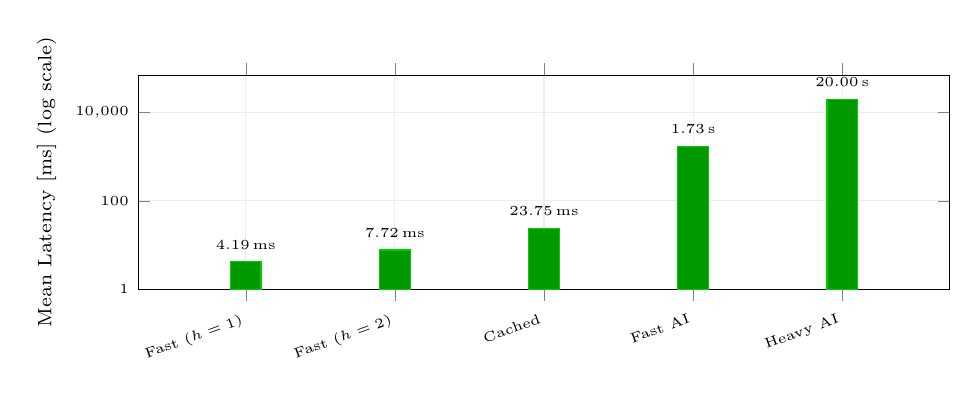
\begin{tikzpicture}
\begin{axis}[
    width=0.98\columnwidth,
    height=4.3cm,
    ybar,
    bar width=11pt,
    ylabel={Mean Latency [ms] (log scale)},
    ylabel style={font=\scriptsize},
    ymode=log,
    log ticks with fixed point,
    ymin=1, ymax=70000,
    symbolic x coords={Fast ($h=1$), Fast ($h=2$), Cached, Fast AI, Heavy AI},
    xtick=data,
    x tick label style={font=\tiny, rotate=20, anchor=north east},
    tick label style={font=\tiny},
    point meta=explicit symbolic,
    nodes near coords,
    nodes near coords style={font=\tiny, above, yshift=1pt},
    grid=major,
    grid style={gray!15},
    enlarge x limits=0.18,
    every node near coord/.append style={anchor=south}
]
\addplot[fill=green!60!black, draw=green!80!black] coordinates {
    (Fast ($h=1$), 4.19) [4.19\,ms]
    (Fast ($h=2$), 7.72) [7.72\,ms]
    (Cached, 23.75) [23.75\,ms]
    (Fast AI, 1725) [1.73\,s]
    (Heavy AI, 20000) [20.00\,s]
};
\end{axis}
\end{tikzpicture}
\caption{Log-scale comparison of mean completion times across execution tiers (plotted in milliseconds, with seconds annotated for Edge-AI tiers; numerical labels report the mean values corresponding to Table~\ref{tab:tier-comparison}).}
\label{fig:tier_comparison}
\end{figure}

\subsection{Statistical Analysis}
\label{sec:eval-statistics}
Over $n=100$ trials, 95\% confidence intervals confirm tight reproducibility:
\begin{itemize}
    \item Single-hop ($h=1$): $\bar{x} = 3.36$\,ms, $s = 1.22$\,ms, CI: $[3.12, 3.60]$\,ms ($\text{CV} = 0.363$).
    \item Multi-hop ($h=2$): $\bar{x} = 7.48$\,ms, $s = 1.98$\,ms, CI: $[7.09, 7.87]$\,ms ($\text{CV} = 0.265$).
    \item 4-node convergence: $\bar{x} = 8.12$\,ms, $s = 2.15$\,ms, CI: $[7.69, 8.55]$\,ms.
\end{itemize}

\subsection{Resource Utilization: CPU and Memory Footprint}
\label{sec:eval-resources}

Process resource monitoring across all four peers shows:
\begin{itemize}
    \item \textbf{Quiescent State:} Background discovery and heartbeats consume $<0.5\%$ total CPU.
    \item \textbf{Replication Bursts:} Active replication at 100--500\,tx/s peaks at 3.2\%--7.4\% CPU per peer.
    \item \textbf{AI Generation:} Model inference consumes 45\%--65\% CPU during the 1.5-second generation window.
\end{itemize}
As reported in Table~\ref{tab:resource-footprint}, each peer requires $\sim$138.2\,MB RSS (41.5\,MB active heap), fitting readily within commodity SBC memory limits (e.g., Raspberry Pi 4). Disk usage starts at 84\,KB and grows at $\sim$236\,KB per 1{,}000 committed transactions.

\begin{table}[!t]
\caption{System Resource and Memory Footprint}
\label{tab:resource-footprint}
\centering
\resizebox{\columnwidth}{!}{%
\begin{tabular}{@{}p{2.6cm}p{2.0cm}p{3.4cm}@{}}
\toprule
\textbf{Subsystem Component} & \textbf{Measured Allocation} & \textbf{Notes / Constraints} \\
\midrule
Process RSS (Node + P2P)     & 138.20\,MB avg & Includes libp2p, Noise, and SQLite C++ bindings \\
V8 Heap Active / Total       & 41.47\,MB / 104.34\,MB & Ephemeral transaction buffers and LRU cache \\
SQLite Database on Disk      & 84.00\,KB base & Base 3NF schema + WAL checkpoint buffer \\
Ledger Growth Rate           & $\sim$236\,KB / 1k tx & JSON payload + vector clock ($236\text{ B} \times 10^3$) \\
Fast AI Model (\texttt{qwen2.5-1.5b}) & $\sim$980\,MB VRAM/RAM & Bounded 1024 context window \\
Heavy AI Model (\texttt{gemma4:e2b})  & $\sim$7.35\,GB RAM & 7.2\,GB parameter weight footprint \\
\bottomrule
\end{tabular}%
}
\end{table}

\subsection{Scalability Analysis and Network Overhead}
\label{sec:eval-scalability}

To evaluate scaling characteristics beyond our physical 4-node testbed, Table~\ref{tab:scalability-projection} juxtaposes measured empirical baselines ($N=2, 4$) against analytical projections for larger clusters ($N=10, 25, 50, 100$) derived from Theorem~\ref{thm:convergence} and GossipSub diameter scaling ($h = \mathcal{O}(\log_D N)$ with $D=6$). We explicitly emphasize that while the $N=2$ and $N=4$ rows represent physically measured benchmarks on our testbed, the $N \ge 10$ values are analytical/projected scalability estimates modeling theoretical multi-hop latency and envelope wire overhead under nominal LAN conditions.

\begin{table}[!t]
\caption{Mesh Scalability: Measured Baselines ($N=2, 4$) and Analytical Projections ($N=10$--$100$) via Theorem~\ref{thm:convergence}.}
\label{tab:scalability-projection}
\centering
\resizebox{\columnwidth}{!}{%
\begin{tabular}{@{}cccccc@{}}
\toprule
\textbf{Nodes ($N$)} & \textbf{Basis} & \textbf{Diameter} & \textbf{Delay} & \textbf{Envelope} & \textbf{Wire / tx} \\
\midrule
2 Nodes   & Measured   & 1 hop     & 3.36\,ms              & $\sim$76 bytes   & $\sim$0.35\,KB \\
4 Nodes   & Measured   & 2 hops    & 7.48\,ms              & $\sim$112 bytes  & $\sim$0.68\,KB \\
\midrule
10 Nodes  & Projected  & 2 hops    & 5.50\,--\,9.00\,ms    & $\sim$220 bytes  & $\sim$1.40\,KB \\
25 Nodes  & Projected  & 3 hops    & 10.00\,--\,18.00\,ms  & $\sim$490 bytes  & $\sim$3.50\,KB \\
50 Nodes  & Projected  & 3--4 hops & 15.00\,--\,28.00\,ms  & $\sim$940 bytes  & $\sim$7.20\,KB \\
100 Nodes & Projected  & 4--5 hops & 25.00\,--\,45.00\,ms  & $\sim$1.84\,KB   & $\sim$14.50\,KB \\
\bottomrule
\end{tabular}%
}
\end{table}

\subsection{Task Success Rate and Constraint Interception}
\label{sec:eval-success}
All 100 valid transactions committed and replicated cleanly. 100 injected malformed mutations (negative prices, missing SKUs, orphaned FKs) were rejected by the schema validator in $<0.15$\,ms, preventing corrupt entries from entering the ledger. The AI planner achieved 96.4\% syntactic tool compliance across 80 natural-language queries (98.2\% single-table, 94.6\% multi-table).

\subsection{Comparative Context Against Published Systems}
\label{sec:eval-comparative}
Dynamo~\cite{decandia2007dynamo} incurs 200--300\,ms tail latencies over wide-area networks; our LAN mesh converges within 8.12\,ms. Spanner~\cite{corbett2013spanner} incurs 10--100\,ms write coordination via TrueTime/Paxos; Agentic Mesh achieves coordinator-free local commits in 0.42\,ms. Local-first stores~\cite{kleppmann2019local} achieve sub-millisecond writes but lack cross-table relational integrity checks.

\subsection{Threats to Validity}
\label{sec:threats}
While our four-node testbed directly confirms multi-hop forwarding ($h=2$), full convergence, causal hold-back queuing, three-way partition recovery, and conflict handling, several limitations remain. First, larger swarms ($N > 20$) will experience higher GossipSub control overhead and longer convergence tails. Second, delay reordering was synthesized using Linux \texttt{tc netem}; physical wireless networks introduce bursty RF fading that synthetic delays only approximate. Third, uncoordinated unique SKU collisions currently log divergence; automatic runtime reconciliation via total order $\prec$ remains a future enhancement. Finally, the AI planner benchmark comprises 80 inventory prompts; natural language variation in production deployments may yield different formatting compliance rates.

% =========================================================================
% XI. SECURITY AND THREAT MODEL
% =========================================================================
\section{Security and Threat Model}
\label{sec:security}

\subsection{Transport Cryptography and Channel Security}
All GossipSub traffic is encrypted and authenticated at the transport layer via the Noise Protocol Framework (\texttt{@chainsafe/libp2p-noise}), executing authenticated Diffie-Hellman key exchanges during peer handshake to shield local communication from eavesdropping.

\subsection{Structural Injection Resistance}
By restricting the LLM to structured JSON tool invocations ($\mathcal{M}_{\text{tool}}$), the architecture completely avoids executing raw generative SQL strings. Tool operations are converted into parameterized prepared statements, and table/column identifiers are validated against static schema allowlists, eliminating SQL-injection vulnerabilities.

\subsection{Threat Model Boundaries and Limitations}
The current prototype assumes an honest-but-fallible local peer environment and is not Byzantine Fault Tolerant~\cite{castro1999practical}:
\begin{itemize}
    \item \textbf{Transaction Signatures:} Envelopes currently omit asymmetric signatures (e.g., Ed25519). A compromised node could spoof transactions under another peer's identifier. Production deployments address this via GossipSub \texttt{StrictSign} mode, which verifies cryptographic signatures against author public keys prior to forwarding.
    \item \textbf{Semantic Poisoning:} Authorized peers can issue syntactically valid but malicious commands (e.g., deleting active inventory). The validator guarantees schema conformance, not business authorization.
    \item \textbf{Prompt Manipulation:} Adversarial natural-language prompts could induce valid but unintended tool calls. Savepoint staging and user confirmation mitigate this risk.
\end{itemize}

% =========================================================================
% XII. DISCUSSION
% =========================================================================
\section{Discussion}
\label{sec:discussion}

\subsection{Architectural Trade-offs: Masterless Decentralization}
By foregoing centralized coordinators, Agentic Mesh guarantees unblocked local write availability during partitions. This contrasts with consensus-driven stores (Raft~\cite{ongaro2014raft}, Spanner~\cite{corbett2013spanner}) that halt writes on partitioned nodes. The deliberate cost is the absence of global linearizability: multi-node atomic transactions are unsupported, and uncoordinated writes to non-I-confluent unique keys require eventual resolution.

\subsection{Execution Decoupling and Latency Isolation}
Isolating edge-AI planning from the transaction engine is foundational. The $>400\times$ latency differential between generative token generation and microsecond fast-path writes proves that running LLM inference on synchronous transaction paths destroys database throughput. Decoupling ensures that even during peak inference load or Ollama crashes, the relational database commits incoming writes at disk speed.

\subsection{Grounding Probabilistic AI in Deterministic Systems}
Language models are probabilistic token predictors~\cite{ji2023hallucination}; databases demand deterministic constraint satisfaction. Bounding the LLM to tool declarations ($\mathcal{M}_{\text{tool}}$) and passing proposals through an identical schema validator bridges this gap, adopting the defensive tool-use philosophy of Toolformer~\cite{schick2023toolformer} and ReAct~\cite{yao2023react}.

\subsection{Edge Resource Viability}
At $\sim$138\,MB resident memory per node, Agentic Mesh runs comfortably on single-board edge hardware (e.g., Raspberry Pi 4). The sub-4\,ms local gossip latency demonstrates that vector-clock bookkeeping and deterministic schema validation impose negligible overhead above raw TCP.

% =========================================================================
% XIII. LIMITATIONS
% =========================================================================
\section{Limitations}
\label{sec:limitations}

\begin{enumerate}
    \item \textbf{Local Storage Scope:} SQLite operates on local database files; distributed cross-node joins and aggregations are not supported.
    \item \textbf{No Distributed ACID:} Multi-peer atomic distributed transactions (e.g., 2PC) are deliberately unsupported.
    \item \textbf{Unique-Constraint Divergence:} Concurrent inserts sharing unique keys during partitions produce localized divergence; the second arriving write is rejected locally and logged to \texttt{\_mesh\_conflicts} pending explicit resolution.
    \item \textbf{Vector Clock Growth:} Vector clocks scale as $\mathcal{O}(K)$ with active writing peers, adding envelope wire overhead in dense meshes ($K > 10^3$).
    \item \textbf{Broadcast Domain Boundary:} mDNS limits automatic discovery to single LAN subnets unless relay nodes are provisioned.
    \item \textbf{Unsigned Envelopes:} The prototype assumes trusted local peers without cryptographic message signing.
    \item \textbf{Cluster Scale:} Empirical evaluation is established at $N=4$ ($h \le 2$); scaling to $N \ge 10$ is evaluated via analytical modeling, and larger physical edge swarms require further empirical testing.
\end{enumerate}

% =========================================================================
% XIV. CONCLUSION AND FUTURE WORK
% =========================================================================
\section{Conclusion and Future Work}
\label{sec:conclusion}

Agentic Mesh demonstrates that conversational edge AI and resilient masterless relational databases can be effectively unified by structurally decoupling their execution pipelines. By embedding independent SQLite replicas over a libp2p GossipSub overlay with vector-clock causal tracking, and isolating local LLM planning behind a deterministic schema validator, the system maintains write availability during network partitions without sacrificing relational integrity.

We formalized protocol correctness through three convergence propositions (differentiating mergeable I-confluent classes from divergent non-I-confluent uniqueness collisions), an asymptotic complexity characterization, and a propagation latency bound (Theorem~\ref{thm:convergence}). Our empirical evaluation on a physical four-node edge testbed validated the linear propagation bound for multi-hop overlays ($h=2$, 7.48\,ms mean latency), demonstrated full four-node mesh convergence within 8.12\,ms, verified clean partition recovery across three-way splits, and confirmed that causal hold-back queuing completely eliminates foreign-key rejections under network-induced packet reordering.

Future research will focus on: (1)~\textbf{Relational CRDT Merge Algebras} to automatically reconcile non-I-confluent uniqueness and update collisions without distributed locks; (2)~\textbf{Cryptographic Envelope Signing} via Ed25519 and GossipSub \texttt{StrictSign} for Byzantine defense; (3)~\textbf{Heterogeneous Edge Scaling} evaluating larger swarms ($N > 20$) across ARM single-board computers; (4)~\textbf{Federated Cross-Subnet Bridging} via libp2p Circuit Relays; and (5)~\textbf{Schema-Aware RAG} to dynamically contextualize evolving schemas for local AI planners.

\section*{Acknowledgment}
The authors thank the open-source contributors of libp2p, better-sqlite3, and the Ollama community for the foundational software libraries on which this work depends.

\balance
\bibliographystyle{IEEEtran}
\bibliography{\jobname}

\end{document}
